\documentclass[a4paper, 12pt]{bxjsreport}
\usepackage{fontspec}
\usepackage{zxjatype}
\usepackage{amsmath} % 数式コマンドの拡張
\usepackage{amssymb} % 追加の数学記号
\usepackage{amsfonts} % 数学フォント(\mathbb 用)
\usepackage{siunitx} % SI単位系
\usepackage{autobreak}
\usepackage{bm}
\usepackage[dvipdfmx]{graphicx}
\usepackage{float}
\usepackage{cite}
\usepackage{enumerate}
\usepackage[notransparent]{svg}
\usepackage{graphicx}   % 画像を扱うパッケージ
\usepackage{subcaption} % サブキャプションを扱うパッケージ
\geometry{left=25truemm, top=10truemm, right=25truemm, bottom=20truemm}
\setjamainfont{ipam.ttf}
\setjasansfont{ipag.ttf}

\makeatletter
\newcommand{\biggg}[1]{{\hbox{$\left#1\vbox to 20.5pt{}\right.\n@space$}}}
\newcommand{\Biggg}[1]{{\hbox{$\left#1\vbox to 23.5pt{}\right.\n@space$}}}
\newcommand{\ctext}[1]{\raise0.2ex\hbox{\textcircled{\scriptsize{#1}}}}

\begin{document}

\begin{titlepage}
    \begin{center}

        \includesvg[width=110pt]{RIKKYOAI_main.svg}

        \vspace{50truept}

        %%%%%%%%% 修論は以下 %%%%%%%%%
        % {\headfont \Large 2024年度 修士論文}
        % \vspace{20truept}

        % {\headfont \Huge タイトル}
        % \vspace{160truept}
        
        % {\headfont \Large 学籍番号  \LARGE 著者名}
        % \vspace{10truept}
        % % 複数著者の場合は上2行を複製

        % \vspace{20truept}

        % {\headfont \Large 指導教員  指導教員名}
        % % 複数教員の場合、「\and」 でつなげる
        %%%%%%%%%%%%%%%%%%%%%%%%%%%%%

        %%%%% プロジェクト実習は以下 %%%%%
        {\headfont \Large 2024年度 修士論文}
        \vspace{20truept}

        {\headfont \Huge 津波避難誘導のマルチエージェント強化学習ドローンによるアプローチの検討}
        \vspace{160truept}
        
        {\headfont \Large 23VR008N  \LARGE 高林 秀}\\ \vspace{10truept}
        % 著者が増える場合は上行を複製
        
        \vspace{20truept}

        {\headfont \Large 指導教員  三宅陽一郎}
        % 複数教員の場合、「\and」 でつなげる
        %%%%%%%%%%%%%%%%%%%%%%%%%%%%%%%%
        
        \vspace{100truept}
        % ページがはみ出す場合はこの数字を調整

        {\headfont \Large 立教大学大学院}
        
        \vspace{10truept}
        
        {\headfont \Large 人工知能科学研究科 人工知能科学専攻}

    \end{center}
\end{titlepage}

% ===概要===
\begin{abstract}
ここに概要を書く~\cite{sample}
\end{abstract}

% ===目次===
\setcounter{tocdepth}{2}
 % 目次に表示する階層(必要に応じて変更)
 % 0はchapterまで、1でsectionまで、2でsubsectionまで...
\tableofcontents
% ===目次をページ数に入れない===
\thispagestyle{empty}
\clearpage
\addtocounter{page}{-1}

% ===本文(直書きでも可)===
% この方法ではFile outlineが出ない
\chapter{はじめに}
本章では,本論文の要旨および構成について述べる.
\section{要旨}
首都直下型地震や南海トラフ地震をはじめとする,大地震の 30 年以内の発生確率が 70\%~
80\%と非常に高くなっていることに加え,近年の豪雨など,将来の大規模災害のリスクが著
しく高まっている現状がある.
\section{本稿の構成}
まず,第2章において本稿の内容を理解するのに必要な事前知識,研究背景について述べる.
具体的には,以下の項目について説明する.
\begin{itemize}
  \item 強化学習についての基本説明
  \item マルチエージェントアルゴリズム MA-POCA(MultiAgent POsthumous Credit Assignment)について
  \item 本研究の社会的背景・課題について
\end{itemize}

次の第3章においては,本研究の研究手法についての説明を行う.
第4章では,マルチエージェント強化学習エージェントによる,津波避難誘導のシミュレーション実験の結果と考察を行う.
第5章では,実験結果をまとめ,本研究の応用, 今後の研究の展望を述べる.

\chapter{研究背景}

本研究を理解する上で必要な概念である, 強化学習とそのアルゴリズムであるMA-POCAの理論や,関連する研究について述べる.
また,本研究を行うことになった社会的背景についても述べる.

\section{津波避難誘導における課題}
本章では,我が国での津波避難誘導における課題について取り上げ,後述する提案手法の研究背景の理解を補助するものとする.\par 

災害大国である我が国において,地震発生後の津波避難誘導オペレーションは非常に重要である.
% TODO:津波避難オペレーションの重要性を述べる
また近年,津波以外にも異常気象等による気象災害の激甚化もあり,避難誘導の遂行にあたって,益々その危険性も増していると推察される.\par 

\subsection{訪日観光客数の増加と観光地における避難誘導の課題}
近年の大幅な観光客増加と,観光地における避難誘導の課題,その関連性について述べる.
\paragraph{我が国の観光客数増加}
我が国では,2007年にに観光立国推進基本法\footnote{議員立法により平成18年12月13日に成立し,平成19年1月1日から施行されている.本法律において,観光は21世紀における日本の重要な政策の柱として初めて明確に位置づけられた.}が施行され,国として観光客数の増加が進められてきた.
観光庁の調査によれば,我が国における訪日外国人観光客数は増加の一途を辿っている.下図は観光庁が公開している,2003年から2023年までの訪日外国人観光客数の推移を示したグラフである.
\begin{figure}[H] 
  \centering 
  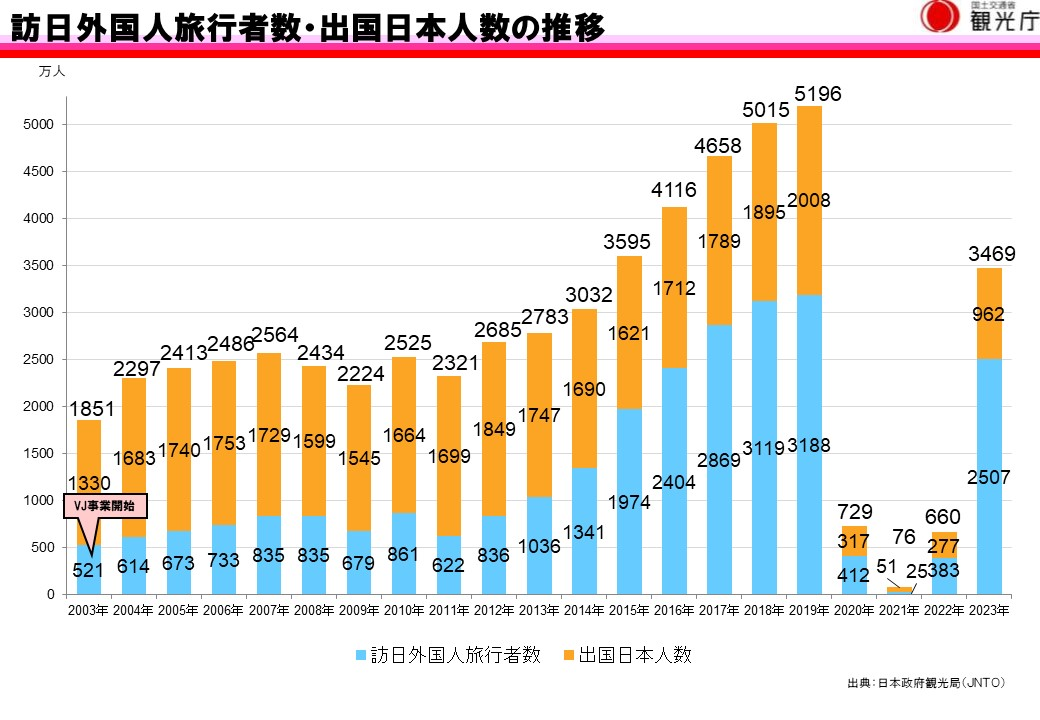
\includegraphics[width=0.8\textwidth]{Figures/001584918.jpg}
  \caption{2003年~2023年の訪日外国人旅行者数の推移} % TODO:いらないかも
  \label{fig:02} 
\end{figure}
上図を読み解くと,2003年から2019年にかけて,訪日外国人観光客数は倍以上に増加していることがうかがえる.2020年から2022年にかけては,著しく観光客数が減少しているが,これは新型コロナウイルスの世界的流行による影響であると考えられる.\par 
また,2023年は新型コロナウイルスによる行動自粛が解除されたことを受け,観光客数は2015年と同等水準まで回復しており,今後も増加するものと推察される.\par 
このような観光客数の急激な増加は,観光地の災害時の避難誘導タスクにおいて,以下のような問題を生じさせ適切な避難誘導を行えない可能性がある.
\begin{itemize}
  \item 観光客の土地勘がないため,的確な避難誘導が必要
  \item 観光客数は時間や季節によって変動するため,特定の避難所に多数の避難者が向かい,収容不足となる可能性がある.
  \item 避難誘導に従わずに周囲の人の動きに追従し,混乱を招く恐れがある.
\end{itemize}

このような,観光客の避難に関する問題は,多くの関連研究でも指摘されている.

\subsection{津波避難タワー・津波避難ビル}
我が国には,津波避難タワーや津波避難ビル\footnote{津波浸水が想定される地域において,地震発生時に住民が一時的,または緊急に避難・退避するための人工施設を言う.
内閣府が2005年に策定した「津波避難ビル等に係るガイドライン」に沿って進められ,2011年の東日本大震災\footnote{2011年3月11日14時46分頃に三陸沖の宮城県牡鹿半島の東南東130km付近を震源とする我が国最大規模の地震災害.}の発生を受け,「津波防災地域づくりに関する法律」によって津波防災対策が制度化された.}が建設されており,津波からの公的な避難先の1つとして提供されている.
\begin{figure}[H]
  \centering
  % 1枚目の画像
  \begin{subfigure}{0.45\textwidth}
      \centering
      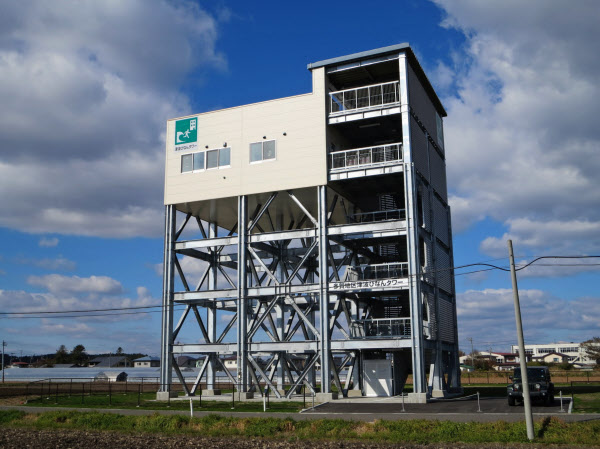
\includegraphics[width=\textwidth]{Figures/https___imgix-proxy.n8s.jp_DSXMZO6372684011092020CC1001-PN1-2.jpg}
      \caption{青森県八戸市の津波避難タワー}
      \label{fig:image1}
  \end{subfigure}
  % 2枚目の画像
  \begin{subfigure}{0.5\textwidth}
      \centering
      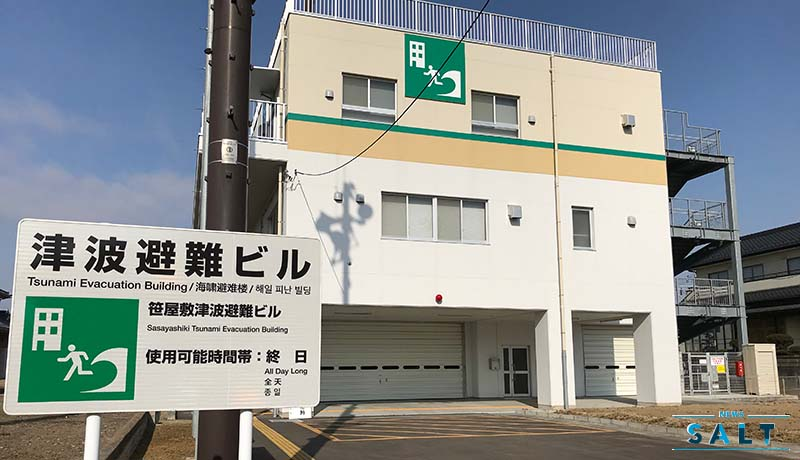
\includegraphics[width=\textwidth]{Figures/20220311_1.jpg}
      \caption{宮城県仙台市の津波避難ビル}
      \label{fig:image2}
  \end{subfigure}
  \caption{}
  \label{fig:side_by_side}
\end{figure}
このような施設の建設にあたっては,避難経路や避難時間などの基準が国から示されており,自治体により適切な位置に建設が進められている.特に,観光地では景観等の問題から,十分な高さの堤防や防波堤を用意することが難しいといった問題もあり,津波避難対策を強化する施策としてこのような津波避難施設の設置は自治体を主導に行われている.
このような施設は,津波から命を守る手段として非常に重要であるが,避難者の行動,配分によっては収容定員を超過し,適切な避難が行えない可能性があることが示されている\cite{kouti-01}.\par 

しかし,その母数が足りず想定される避難者の数をカバーしきれない等の指摘や,被害予測の改訂等で必要な高さ等の基準を満たせていない等の問題も存在する\cite{tsunami_evacuation_koshigoe}.
加えて,ほとんどの観光客は土地勘がないとともに,防災意識もあまり高いとは言えない結果がアンケート調査で判明している.\cite{visitor01}.

このような状況下では,近隣の高台へ避難することが求められるが,土地勘のない観光客や外国人観光客に対してこれを求めるのはかなり難しく,既往研究の多くで指摘されている問題である.\par 

また,観光地特有の問題として一部の避難所に避難者が集中し,避難完了時間が遅くなるというシミュレーション結果が示されており,適切に他の避難所(ないしは避難ビル)に避難者を誘導することの必要性が指摘されている\cite{kitahara2013tsunami}.


\vspace{\baselineskip}
以上の背景から,今後発生しうる,南海トラフ地震などの巨大地震とそれにより発生する津波からの避難に関して,その対策は進められてきてはいるものの,地元住民だけでなく観光客も含めた避難に関しては多くの課題を残している現状がある.
また,避難する人だけでなく,避難者を適切な場所へ誘導する人員の安全確保にも課題が残されている.


\subsection{二次被害の発生}
津波避難誘導(あるいは,他の災害における避難誘導)においては,発災直後から二次被害にあう危険性が高い地域で活動しなければならないため,現場で誘導を行う警察や消防員等の安全確保が問題になっている.\par
\paragraph{風水害時における人的被害の特徴}
以下は,我が国で発生した1969年から2018年までの災害を対象に,消防団員が殉職した事例を消防白書や新聞記事,既往研究などから把握し,殉職時の状況を分析した結果が,山田らの研究\cite{yamada2020}によって報告されている.
\begin{quote}
  図-3 より,津波は,出動 途上,水防作業中,避難中,避難誘導中,人命救助中に 殉職者を出したことがわかった.なかでも避難誘導中と 避難中を合わせると全体で約 80\%を占めており,避難に関係する時に殉職者が出ている.
  \begin{figure}[H] 
    \centering 
    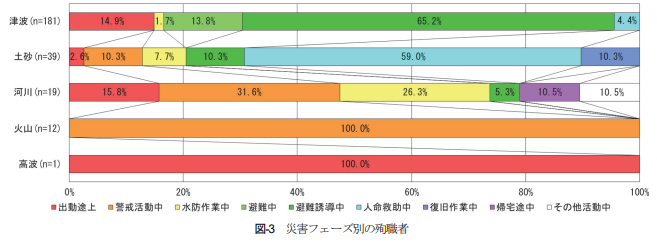
\includegraphics[width=0.8\textwidth]{Figures/fig-01.png}
    \caption{消防団員の災害フェーズ別殉職者の割合} 
    \label{fig:01} 
  \end{figure}
\end{quote}
以上より,津波災害時の消防団員おけるの2次被害に関しては,避難誘導中が最も多い結果であることが示されている.上記は消防団員に限定した統計であるが,同じく避難誘導を行うすべての人員においても同様の傾向があると推察される.\par
また,東日本大震災のケースにおいても,避難誘導にあたった警察職員や自治体職員の多数が地域住民の避難誘導中に津波に巻き込まれ殉職された事例\cite{touhoku-01}が報告されており,このような二次被害の防止は避難誘導において重要な意味を持つ.

\section{既存のドローンの災害対応における活用事例と航空法改正}
加えて,我が国では,2022年に航空法が改正され,これまで規制されていたドローンの有人地帯目視外飛行(レベル4飛行\footnote{無人機の運用・操縦方法をレベル別に定めたもの.レベル4では操縦者が直接目視で機体を見ていなくても有人地帯でドローンを飛ばすことが可能になった.})が解禁された.
これにより,これまでドローンの活用が規制されていた防災分野での利活用や研究が大きく進んだ背景がある.\par 
\begin{table}[H]
  \centering
  \begin{tabular}{|l|lll|}
  \hline
       & 操縦方法 & 視界         & 飛行可能場所  \\ \hline
  レベル1 & 操縦飛行 & 目視内        & 無人/有人地帯 \\ \hline
  レベル2 & 自律飛行 & 目視内        & 無人/有人地帯 \\ \hline
  レベル3 & 自律飛行 & 目視外(補助者無し) & 無人地帯    \\ \hline
  レベル4 & 自律飛行 & 目視外(補助者無し) & 有人地帯    \\ \hline
  \end{tabular}
  \caption{ドローンの飛行レベル別概要}
\end{table}
近年我が国では,少子高齢化に伴う労働人口の減少の問題もあり,災害対応人材の不足が懸念されている背景がある.そのような人手不足に対応するため,ドローン等による災害対応の機械化・省人化が進められ始めている.
総務省・消防庁が公開しているデータ\cite{soumusho-01}によると,全国の消防本部におけるドローンの活用率は年々上昇しており,2017年には9.6\%だったものが,2021年には52.9\%と全国半数以上の消防本部でドローンの利活用が進めらたことが報告されている.
\begin{figure}[H] 
  \centering 
  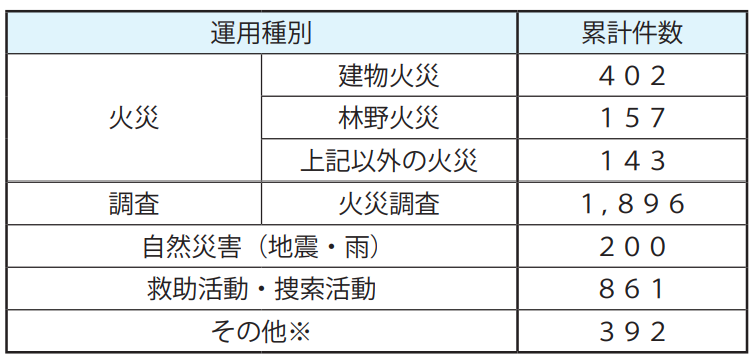
\includegraphics[width=0.6\textwidth]{Figures/2024-11-28 215911.png}
  \caption{ドローンの運用種別ごとの累計活用件数} 
  \label{fig:01} 
\end{figure}



\subsection{ドローンによる避難誘導の先行研究と自治体の実証実験の事例}
ドローンを初めとするUAVの津波避難誘導に置ける活用方法を検討した既往研究が存在する。
杉安らの研究では、津波避難時の迅速な避難行動を促進するために、UAV(無人航空機)の活用可能性を示し,避難誘導を視覚的に行うことを目的とし、福島県いわき市を対象に実証実験を行っている\cite{sugiyasu2018uav}.

また、本研究と関連する先行研究事例として,鈴木らが行った協調ドローンを用いた避難誘導支援システムの研究がある\cite{suzuki2020drone}.この研究では,ドローンを活用して,安全な避難経路を生成し,被災者を誘導するシステムを提案している.
被災者はARマーカーを身に着け、ドローンがこれを識別することで位置情報を取得し,後述するa*アルゴリズムにより避難経路を探索し,計算した軌道情報に沿って対象者を誘導するものである.この研究では実機による誘導試験も行っており,ドローンによる避難誘導の実現可能性を示した。
もう一つの先行研究事例として、複数のドローンが連携して避難誘導を行うことを検証した高橋らの研究が存在する\cite{takahashi2018uav}。この研究では、自然災害時にUAV(無人航空機)を活用して避難誘導を行う支援システムの設計と試作について述べている.
このシステムは複数のUAVが連携して避難者を誘導する仕組みを構築しており、沿岸部地域を対象にした実証実験まで行っている. UAVエージェントによる避難誘導プラン生成と経路選択,複数の UAV の協調による避難誘導機能の実現可能性が示された.\par

また,改正航空法の施行後,沿岸部の自治体を中心に,津波避難誘導を行うドローンの研究や実証実験が進められている.
宮城県仙台市では,東日本大震災の際に津波避難誘導を行っていた自治体職員が津波に巻き込まれ犠牲になった事例を受け,津波避難を呼びかける手段として津波避難広報ドローンの研究が行われている\cite{sendai_tsunami_drone}.この実証実験は,「自動運航のドローンにより津波避難広報を行うこと」及び「専用のLTE通信網でドローンの制御等を行うこと」の2点において世界初の事例で,
Jアラート\footnote{全国瞬時警報システム(Jアラート)とは,弾道ミサイル情報,緊急地震速報,大津波警報など,対処に時間的余裕のない事態に関する情報を携帯電話等に配信される緊急速報システム}による津波情報を受信した後,飛行経路上の気象条件を確認し自律的にドローンの飛行可否を判断した後,事前に定められた飛行ルート上を飛行しながら津波避難のアナウンスを行うというものである.
また,ドローンの管制システムには専用のLTE通信網を利用しており,令和4年10月に整備を完了し本格運用に入っている.\par


以上の様に、ドローンを用いた避難誘導システムの基礎研究や、自治体による避難誘導案内ドローンの整備など、災害時の避難誘導においてドローンの活用が検討,実装が進められている。\par

ただし、これらの研究事例においては,後述する提案手法で示す,本研究が行うような要避難者の位置分布に基づいた各ドローンの配置や移動,避難先の収容人数を考慮した避難誘導の最適化は行われていない.
これらの点を後述する提案手法の章にて、本研究が示す新規性として具体的に述べる.

\section{強化学習}
強化学習とは,エージェント\footnote{モデルを訓練するための主体.環境に対して行動を出力する.}と環境\footnote{エージェントがいる世界,モデルの訓練を行うための様々な機能や状態を提供する.}との相互作用を通じ,
得られる報酬\footnote{エージェントの行動の良し悪しを判断する評価値.行動に対する環境からの評価}を最大化するエージェントの方策\footnote{ポリシーとも呼ばれる.環境の状態に基づいて,次の行動を決定するための
ルール}を学習する機械学習アルゴリズムの種類である.
\begin{figure}[H] 
  \centering 
  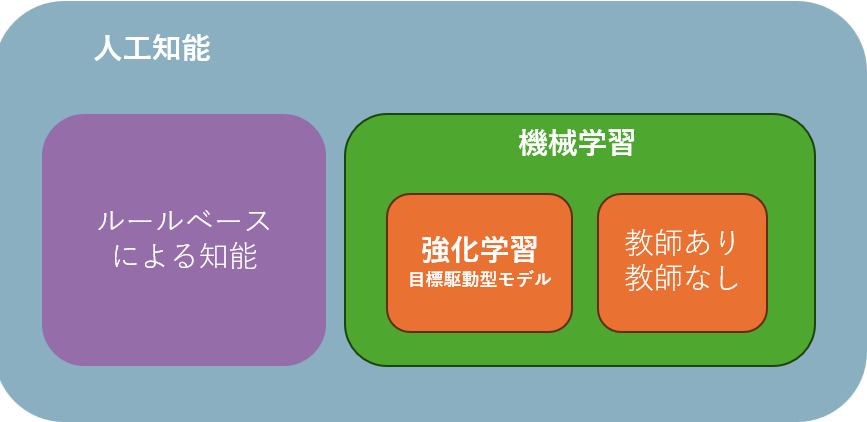
\includegraphics[width=0.6\textwidth]{Figures/2024-12-09 202235.png}
  \caption{強化学習の枠組み概念図} 
  \label{fig:01} 
\end{figure}
教師あり学習・教師なし学習のデータ駆動型機械学習モデルと異なり,事前に訓練データを作成する必要はなく,訓練に必要なデータはエージェントが環境から得るものである.強化学習は与えられた環境の中で,最適な戦略行動 (方策)を分析することが目的となる.
このような特性から,強化学習は目的駆動型モデルや行動駆動型モデルと呼ばれることもある.
エージェントの一連の流れである「観測」,「行動出力」,「報酬獲得」のサイクルを決定と呼ぶ.
\subsection{マルチエージェント強化学習の基本概念}

マルチエージェント強化学習 (Multi-Agent Reinforcement Learning, MARL) では,複数のエージェントが環境と相互作用し,それぞれが自身の行動方策を学習しながら,協調または競争を行う.以下にその基本的な数式を示す.

\subsection*{環境の定義}
環境は,部分観測可能マルコフ決定過程 (Decentralized-POMDP) として定義される:
\[
\mathcal{M} = \langle N, S, \{O_i\}_{i=1}^N, \{A_i\}_{i=1}^N, P, r, \gamma \rangle
\]
ここで:
\begin{itemize}
    \item $N$:エージェントの数
    \item $S$:環境の状態空間
    \item $O_i$:エージェント$i$の観測空間
    \item $A_i$:エージェント$i$の行動空間
    \item $P(s' | s, \boldsymbol{a})$:状態$s$と行動の組み合わせ$\boldsymbol{a} = (a_1, a_2, \dots, a_N)$から次の状態$s'$への遷移確率
    \item $r(s, \boldsymbol{a})$:共有報酬関数
    \item $\gamma$:割引率
\end{itemize}

\subsection*{エージェントの行動方策}
各エージェント$i$は,観測$O_i$に基づき行動を選択する方策$\pi_i(a_i | o_i)$を学習する.エージェント全体の方策は次のように表される:
\[
\pi(\boldsymbol{a} | \boldsymbol{o}) = \prod_{i=1}^N \pi_i(a_i | o_i)
\]

\subsection*{状態価値関数と行動価値関数}
\begin{itemize}
    \item 状態価値関数$V^\pi(s)$は,状態$s$から始まり方策$\pi$に従ったときの期待累積報酬である:
    \[
    V^\pi(s) = \mathbb{E}_\pi \left[ \sum_{t=0}^\infty \gamma^t r(s_t, \boldsymbol{a}_t) \mid s_0 = s \right]
    \]
    \item 行動価値関数$Q^\pi(s, \boldsymbol{a})$は,状態$s$で行動$\boldsymbol{a}$を取った場合の期待累積報酬である:
    \[
    Q^\pi(s, \boldsymbol{a}) = r(s, \boldsymbol{a}) + \mathbb{E}_\pi \left[ \sum_{t=1}^\infty \gamma^t r(s_t, \boldsymbol{a}_t) \right]
    \]
\end{itemize}

\subsection*{集中化されたCritic}
MARLでは,集中化されたCriticを用いて全エージェントの観測$\boldsymbol{o}$と行動$\boldsymbol{a}$を基に価値関数を近似する:
\[
Q^\pi(s, \boldsymbol{a}) = f_\phi(s, \boldsymbol{a})
\]
ここで$f_\phi$はパラメータ$\phi$を持つ関数近似器(通常はニューラルネットワーク)である.

\subsection*{Advantage関数}
アクター・クリティックアルゴリズムでは,Advantage関数を用いて方策の更新を行う:
\[
A^\pi(s, \boldsymbol{a}) = Q^\pi(s, \boldsymbol{a}) - V^\pi(s)
\]

\subsection*{方策の更新}
エージェントの方策は,Advantage関数を最大化するように勾配上昇法で更新される:
\[
\nabla_\theta J(\pi_\theta) = \mathbb{E}_{\pi_\theta} \left[ \nabla_\theta \log \pi_\theta(a | s) A^\pi(s, a) \right]
\]

\subsection*{協調と競争}
協調タスクでは,全エージェントがグループ報酬$r(s, \boldsymbol{a})$を最大化する.一方,競争タスクでは,各エージェントが自分の報酬を最大化する.

\subsection{MA-POCA(MultiAgent POsthumous Credit Assignment)}
  環境内のエージェントの個体数の増減に対応し,エージェント間の協調行動を重んじるようなタスクを学習するのに適しているアルゴリズムがMA-POCA(MultiAgent POsthumous Credit Assignment)\cite{mapoca}である.\par 
  MA-POCAは既存のマルチエージェントアルゴリズムと比較して,以下の特徴を持つ.
  \begin{itemize}
    \item 環境内のエージェント数の増減に対応した学習が可能
    \item エピソード内でエージェントが生成・消滅するタスクや,標準的な協調タスクにおいて,既存手法を大幅に上回る性能を示した
  \end{itemize}
  例えば,実世界で動くようなドローンをエージェントとして,その群衆飛行を考えた時,あるバッテリーが切れたり,故障したりすることが考えられ,エージェントが他のエージェントよりも先に行動不能(早期終了)になる場合が考えられる.
  既存のマルチエージェントアルゴリズムは,エージェントがエピソード\footnote{エージェントが環境と相互作用してタスクを完了するまでの一連のステップのこと.例えば,迷路のスタート地点からゴール地点までの移動がこれに該当する.一方,「ステップ」とは,そのエピソード内でエージェントが1回行動を選択し,環境から報酬と次の状態を受け取る単位時間のことである.}
  終了前に消滅した場合,そのエージェントの行動出力に関係なく状態を固定することでこれを再現する.これを吸収状態と言い,このようにすることでCriticへの入力数を固定したまま学習を行うことが出来るが,同時に無駄な情報を入力しているとも捉えることができ,環境内のエージェント数が多いほどこの問題は顕著に出現することが指摘されている.\par
  早期終了になったエージェントは,与えられたグループ報酬を経験することができない為,自身の行動のグループにおける価値を計算することができない.MA-POCAは,この問題を解消するために提案されたアルゴリズムで,エージェントが早期終了しても価値を伝搬させるアルゴリズムとなっている.\par
  \paragraph{MA-POCAの性能評価}
  MA-POCAは既存のMARL手法よりも多くの場合で性能が向上することが報告されている\cite{mapoca}.
  下記のような4つの実験環境において,マルチエージェント強化学習手法COMA\footnote{},そして,シングルエージェント強化学習手法PPO\footnote{}とMA-POCAの性能を比較した結果が示されている.
  \begin{figure}[H] 
    \centering 
    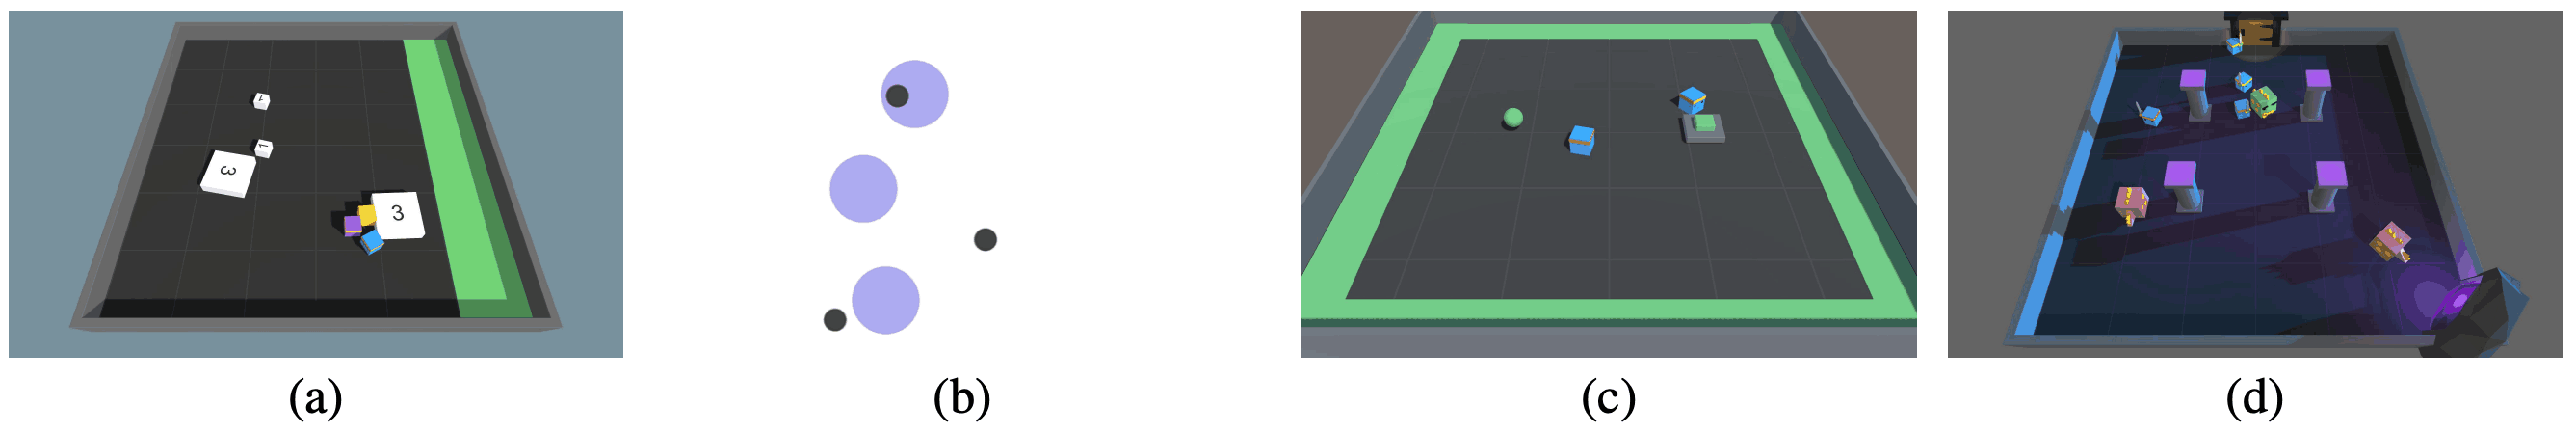
\includegraphics[width=1.0\textwidth]{Figures/2022-10-06_10.03.52.png}
    \caption{MA-POCAの性能評価を実施した環境} 
    \label{fig:01} 
  \end{figure}
  \begin{enumerate}[(a)]
    \item \textbf{Collaborative Push Block}
    エージェント(青,黄,紫)は白いブロックを緑の領域まで押す.大きなブロックはより多くのエージェントが押す必要がある.
  
    \item \textbf{Simple Spread}
    エージェント(紫)は互いにぶつかることなく,ターゲット(黒)をカバーするように移動しなければならない.
    
    \item \textbf{Baton Pass}
    青いエージェントが緑色のfoodをつかみ,緑色のボタンを押すと別のエージェントが生まれ,次のfoodをつかむことができるようになるので,それを繰り返す.
    
    \item \textbf{Dungeon Escape}
    青いエージェントは緑のドラゴンを倒し,そのうちの1人を犠牲にしてカギを出さなければならない.チームメイトは鍵を拾って,ピンクのドラゴンを避けながら,ドアまでたどり着くタスク.
\end{enumerate}
下図は,上記4環境における,累積報酬の推移を示している.このように,MA-POCAは既存のMARL手法よりも多くの場合で性能が向上することが報告されている.
\begin{figure}[H] 
  \centering 
  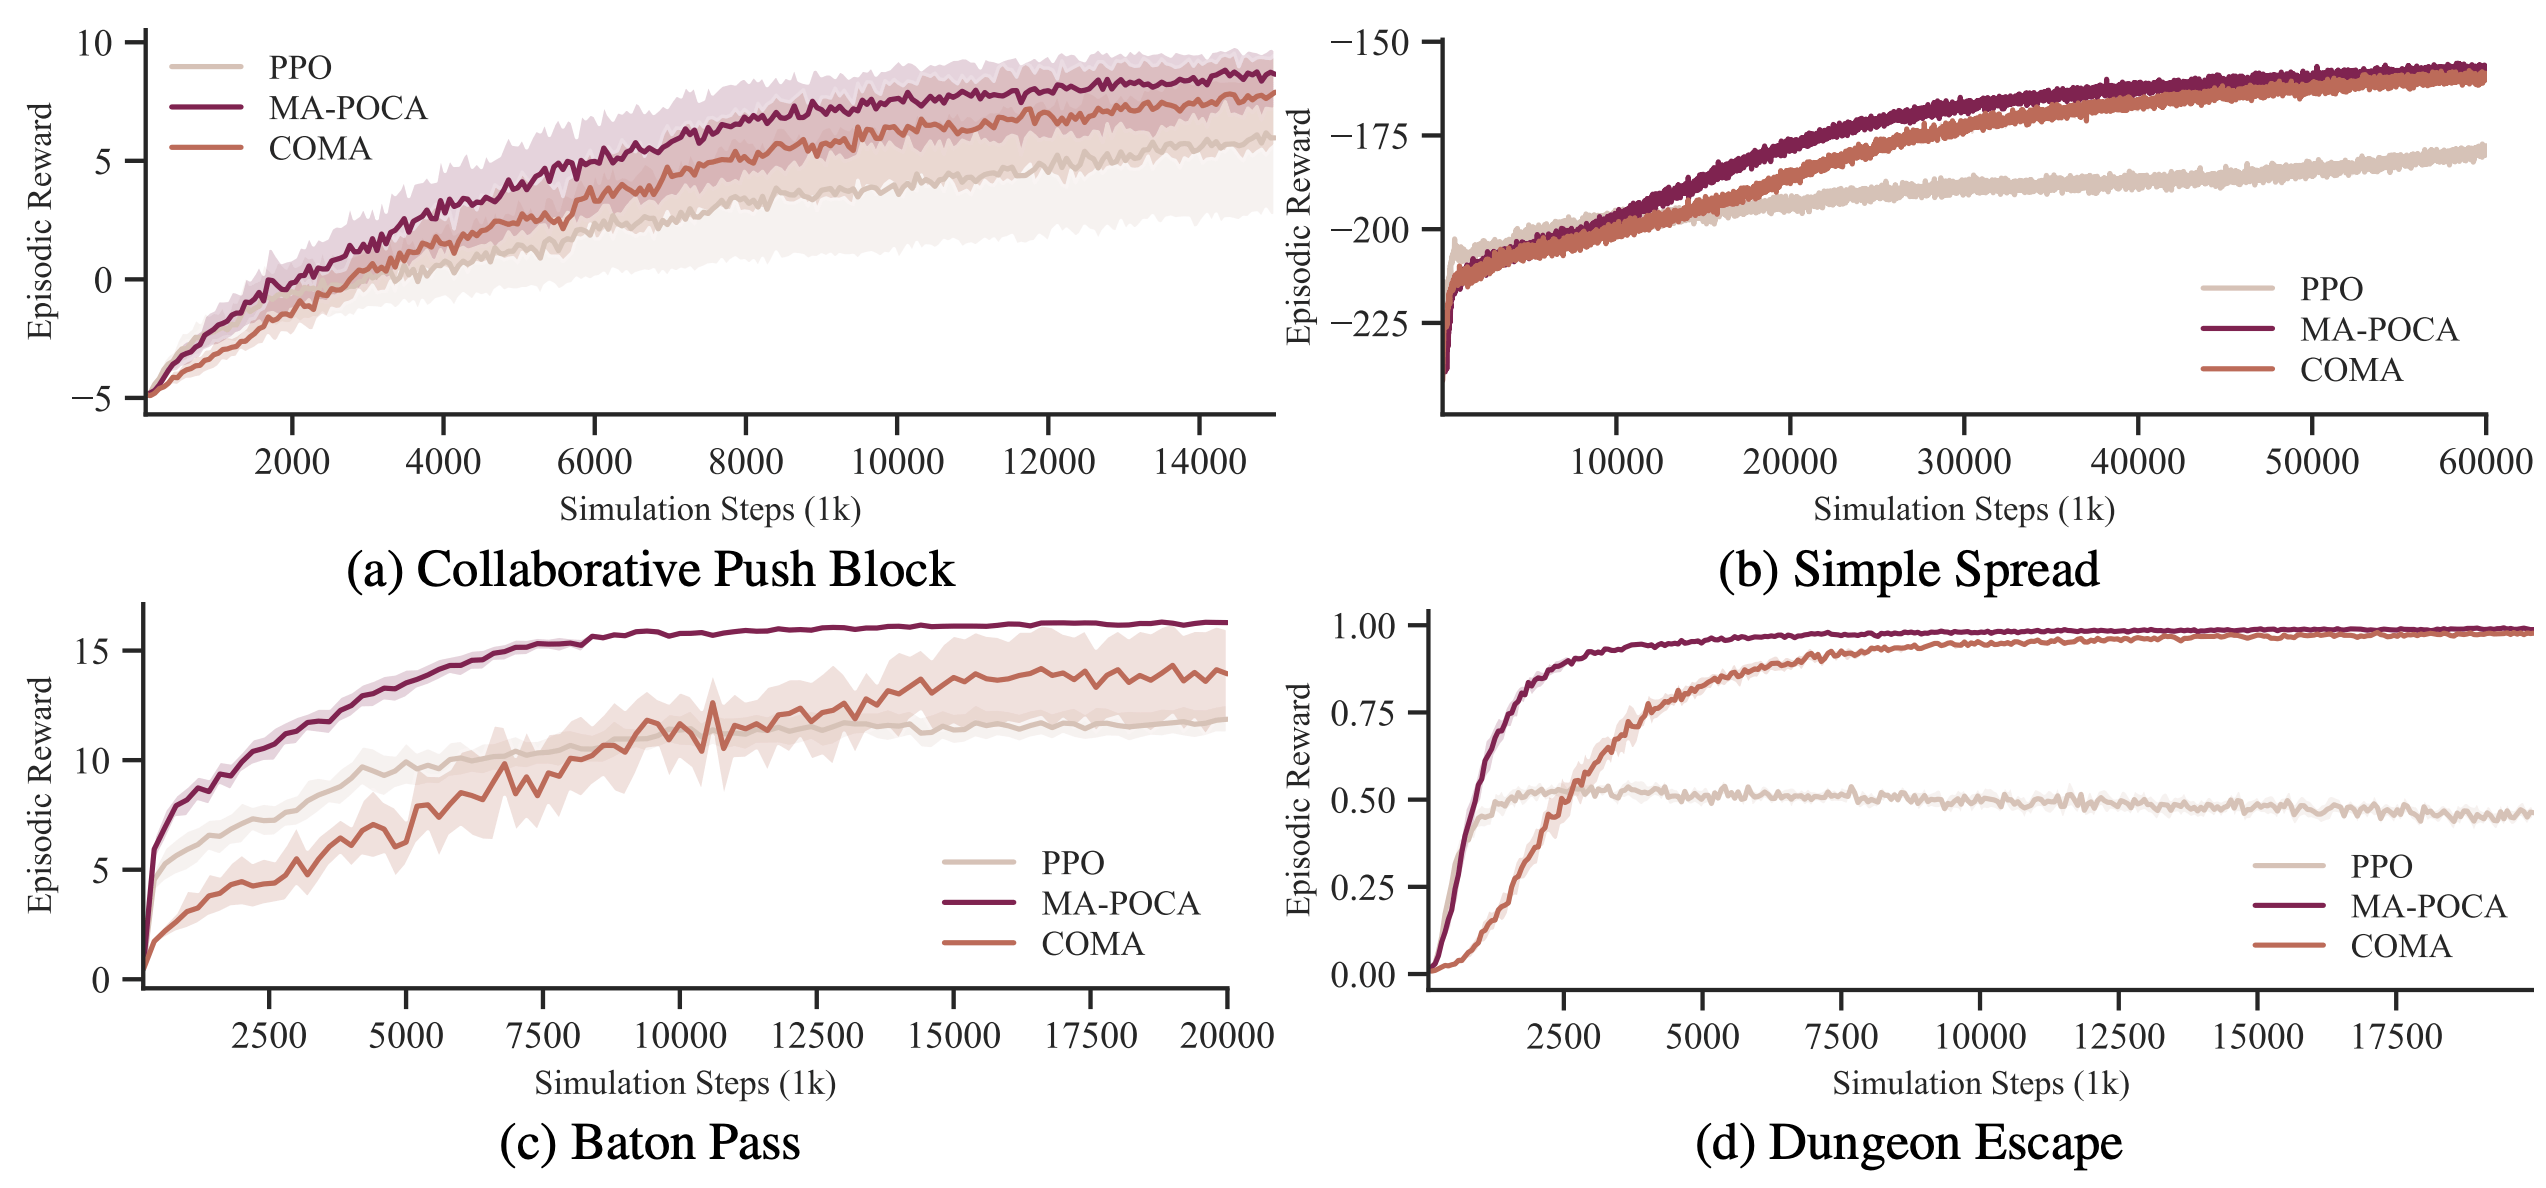
\includegraphics[width=1.0\textwidth]{Figures/2022-10-06_10.04.14-min.png}
  \caption{各環境でのMA-POCAの性能評価結果} 
  \label{fig:01} 
\end{figure}

\section{ナビゲーションメッシュ}
デジタルゲームにおける人工知能\cite{miyake2016}には大きく3つの種類がある.
\begin{itemize}
  \item キャラクターAI : ゲームやシミュレーション内で使用するNPCの頭脳
  \item メタAI : ゲームやシミュレーション全体を監督し,難易度等を調整する
  \item ナビゲーションAI : キャラクターの移動経路検索や障害物等の管理を行う
\end{itemize}

本研究では,エージェントの経路探索に上記のナビゲーションAIに区分される,ナビゲーションメッシュと呼ばれる機能を利用する.
ナビゲーションメッシュは,ノード\footnote{このノードをウェイポイントデータと呼び,ダイクストラ法等のグラフ探索アルゴリズムを用いて最短経路を検索することが可能になる}の連結(グラフ)によって移動可能領域を覆うことで,キャラクターから移動可能範囲,経路を認識させるためのゲームAI技術である.\par
都市モデル上でエージェントを動かす場合,あらゆる経路や移動手段が考えられ,エージェントが移動可能な道路や領域,障害物として認識した上で行動するにはモデル訓練時の経験においてそれらを学習する必要がある.
本研究の目標は,エージェントが避難者を,誘導人数や収容人数等を考慮し適切な避難所へ誘導することが目標なため,ナビゲーションメッシュを使用し事前にエージェントが移動可能な範囲を定めるものとする.


\subsection{a* アルゴリズム}
キャラクターの移動経路を探索するナビゲーション機能のアルゴリズムとしてはa*アルゴリズムが広く利用されている.
a*アルゴリズムは,最短経路を探索するためのグラフ探索アルゴリズムで,経路をノードとして表現しグラフ探索を行う.

スタートノードからゴールノードまでの最短経路を探索する際に,次の評価関数$f(n)$を用いる:
\[
f(n) = g(n) + h(n)
\]
ここで:
\begin{itemize}
    \item $f(n)$: ノード$n$の総評価値.スタートからゴールまでの推定コスト.
    \item $g(n)$: スタートノードから現在のノード$n$までの実際のコスト.
    \item $h(n)$: 現在のノード$n$からゴールノードまでの推定コスト(ヒューリスティック関数).
\end{itemize}

\subsection*{アルゴリズムの手順}
A*アルゴリズムは以下の手順で進行する:
\begin{enumerate}
    \item スタートノードをオープンリストに追加し,初期化する.
    \item オープンリストから$f(n)$が最小のノードを選択する.
    \item 選択したノードがゴールノードであれば,経路探索を終了する.
    \item そのノードの隣接ノードを評価し,以下を実行する:
    \begin{itemize}
        \item 新しいノードであれば,$f(n) = g(n) + h(n)$を計算し,オープンリストに追加する.
        \item 既に評価済みのノードであれば,より低いコストが見つかった場合に更新する.
    \end{itemize}
    \item 評価済みノードをクローズリストに移動し,2に戻る.
\end{enumerate}

\subsection*{ヒューリスティック関数}
ヒューリスティック関数$h(n)$は,A*アルゴリズムの効率と正確性を左右する重要な要素である.一般的な選択肢として以下がある:
\begin{itemize}
    \item マンハッタン距離: 格子状のグラフで利用される.
    \item ユークリッド距離: 2Dまたは3D空間での最短直線距離を近似.
\end{itemize}
$h(n)$が許容可能(ゴールまでの実際のコストを過小評価しない)である場合,A*アルゴリズムは最適解を保証する.

\subsection*{応用例}
A*アルゴリズムは,以下のような応用分野で利用される:
\begin{itemize}
    \item ゲームAI: キャラクターの経路探索.
    \item ロボティクス: 障害物を回避する経路計画.
    \item 地図アプリケーション: 最短経路の検索.
\end{itemize}

\section{強化学習エージェントのデジタルツインへの応用}
デジタルツインとは,現実空間に存在する建物や人流などの情報をリアルタイムで観測し,ネットワーク技術等を使用して仮想空間上に再現する技術のことである.
現実世界と対になる「双子」をデジタル空間上に構築し,モニタリングやシミュレーションを行うことで,社会やビジネスプロセスを進化させることができ,近年注目されている技術分野である.\par 
CRDS\footnote{国立研究開発法人科学技術振興機構 研究開発戦略センター}の調査によると,デジタルツイン関連の研究は,工学分野や計算科学分野を中心として,2016年から2021年の過去5年間の研究論文数で約
30倍に急増しており,米国,ドイツ,英国,中国などでの研究開発が活発であり,各国で大学,公的研究機関,民間企業が連携した研究プロジェクトが推進されていることが報告されている\cite{CRDS2022DigitalTwin}.

デジタルツインと強化学習を組み合わせることで,現実空間で動作するロボットを仮想空間上で強化学習エージェントとして訓練をすることが可能になる.
具体的な事例としては,
Unity\footnote{ユニティ・テクノロジーズ社が開発・提供するゲームエンジン.ゲーム開発の分野で世界シェアナンバー1を誇り,多くのRPGや位置情報ゲーム,VRコンテンツなどが制作可能.}
を活用してロボットのデジタルツインを作成し,強化学習によるトレーニングを行うことで,仮想環境内での動作学習と実世界での性能向上を計るという研究がある\cite{unity_robot_digital_twin_2021}.
また,我が国ではトヨタ自動車株式会社\footnote{愛知県豊田市に本社を置く日本最大手の自動車メーカー.}とSCSK株式会社\footnote{住友商事,住友グループのシステムインテグレータ企業}工場の製造ラインをデジタルツインで再現し,強化学習を活用してロボットの動作や生産プロセスの最適化を目指す取り組みがある\cite{scsk_toyota_digital_twin_2024}.

\subsection{sim2real(Simulation to Reality)}
sim2realとは、デジタル空間内でのシミュレーションで学習したモデルを実世界でモデル適用、並びにタスクに適用する技術のことである。現実空間でエージェントの訓練環境を構築するよりも、デジタル空間でのシミュレーションを用いて訓練を行う方が、手軽に様々な環境条件を設定・試すことができ、低コストでモデルの実装を行うことができる。

一般に、ロボット分野において、シミュレーション上の訓練環境では、状態やその他要因により現実環境を完全に再現することは難しく、モデルの訓練環境と実環境(運用環境)とでギャップが生じる。このギャップが大きいと、エージェントが意図しない動きを行う可能性が高まり、安全上のリスクを伴う。また、モデル訓練時にエージェントが行う試行錯誤による事故や故障のリスクを軽減できる点も、sim2real技術の利点である。\par

sim2real技術を用いてドローンの飛行制御訓練モデルを作成し、現実空間での実機ドローン制御を行った研究がRana Azzamらにより行われた。この研究では、深層強化学習(Deep Reinforcement Learning, DRL)を用いて、動的環境における自律的かつゴール指向型のナビゲーションシステムを開発した。このシステムは、シミュレーション環境でエージェントをトレーニングし、高精度なUAVコントローラーモデルを使用することで、追加のsim2real転送技術なしで現実世界へ適用されている。また、静的および動的障害物を回避しながら、安全かつ効率的にUAVをゴール地点まで誘導することを可能にしている。さらに、現実世界でのテストにおいて90\%の成功率を達成したことが報告されている\cite{azzam2023uav}。

この研究は、消防や救助、監視、物流などのシナリオにおいて、高度な障害物回避機能を備えたリアルタイムのナビゲーションシステムとしての応用が期待されている。また、単一のUAV制御にとどまらず、将来的には複数のUAVの協調制御への拡張も視野に入れている\cite{azzam2023uav}。



デジタルツインと強化学習の融合は,システム設計,運用,制御のすべてにおいて革新的な可能性を提供する.
この組み合わせは,安全性の向上,効率性の最大化,コスト削減を実現し,実世界の複雑な課題に対するソリューションを提供する手段として,今後ますます重要性を増していくだろう.製造業,建築設備,ロボット工学,モビリティ制御など,広範な分野での応用が期待される中,これらの技術が社会全体にもたらす恩恵は計り知れない.

%\subsection{スマートシティへのAIの応用}

%TODO:{三宅先生著:スマートシティへのデジタルゲーム AI の応用}
\chapter{提案手法と実験概要}  
本章では,本研究が最終的に目指す津波避難誘導問題への解決策として,マルチエージェント強化学習と自律飛行型ドローンを組み合わせた提案手法について述べる.
また,提案手法が既存研究と異なる点や新規性についても論じる.

\section{提案手法の概要} 
\label{sec:sug} 
本研究では,観光地や都市部といった地元住民以外にも多数の人々が屋外に存在する状況を想定している.
これには,日常的に避難訓練を受けていない観光客や土地勘のない訪問者も含まれる.
このような状況や,前章で述べた避難誘導における課題を背景に,地震発生後の津波避難という非常に緊急性の高い場面を想定し,避難誘導を行うための手法を検討する.
従来,自治体職員や警察・消防隊員といった人間が担ってきた避難誘導を,自律飛行型ドローンが代替するシステムを構築することを目標とする.

具体的には,マルチエージェント強化学習を活用し,複数のドローンエージェントが協調して行動する能力を学習させることで,刻々と変化する被災地域の状況を動的に認識し,群衆の避難完了率を最大化することを目指す.
また,避難者の位置,避難経路上の障害物,各ドローンの位置などをリアルタイムに反映するデジタルツイン環境を構築し,その環境内で学習済みのエージェントがシミュレーションを通じて最適な誘導方法を実行できるようにする.
%さらに,デジタルツイン環境と実機ドローンを連動させることで,現実世界での運用を可能とする動的な避難誘導システムを構築.

\begin{figure}[H] 
  \centering 
  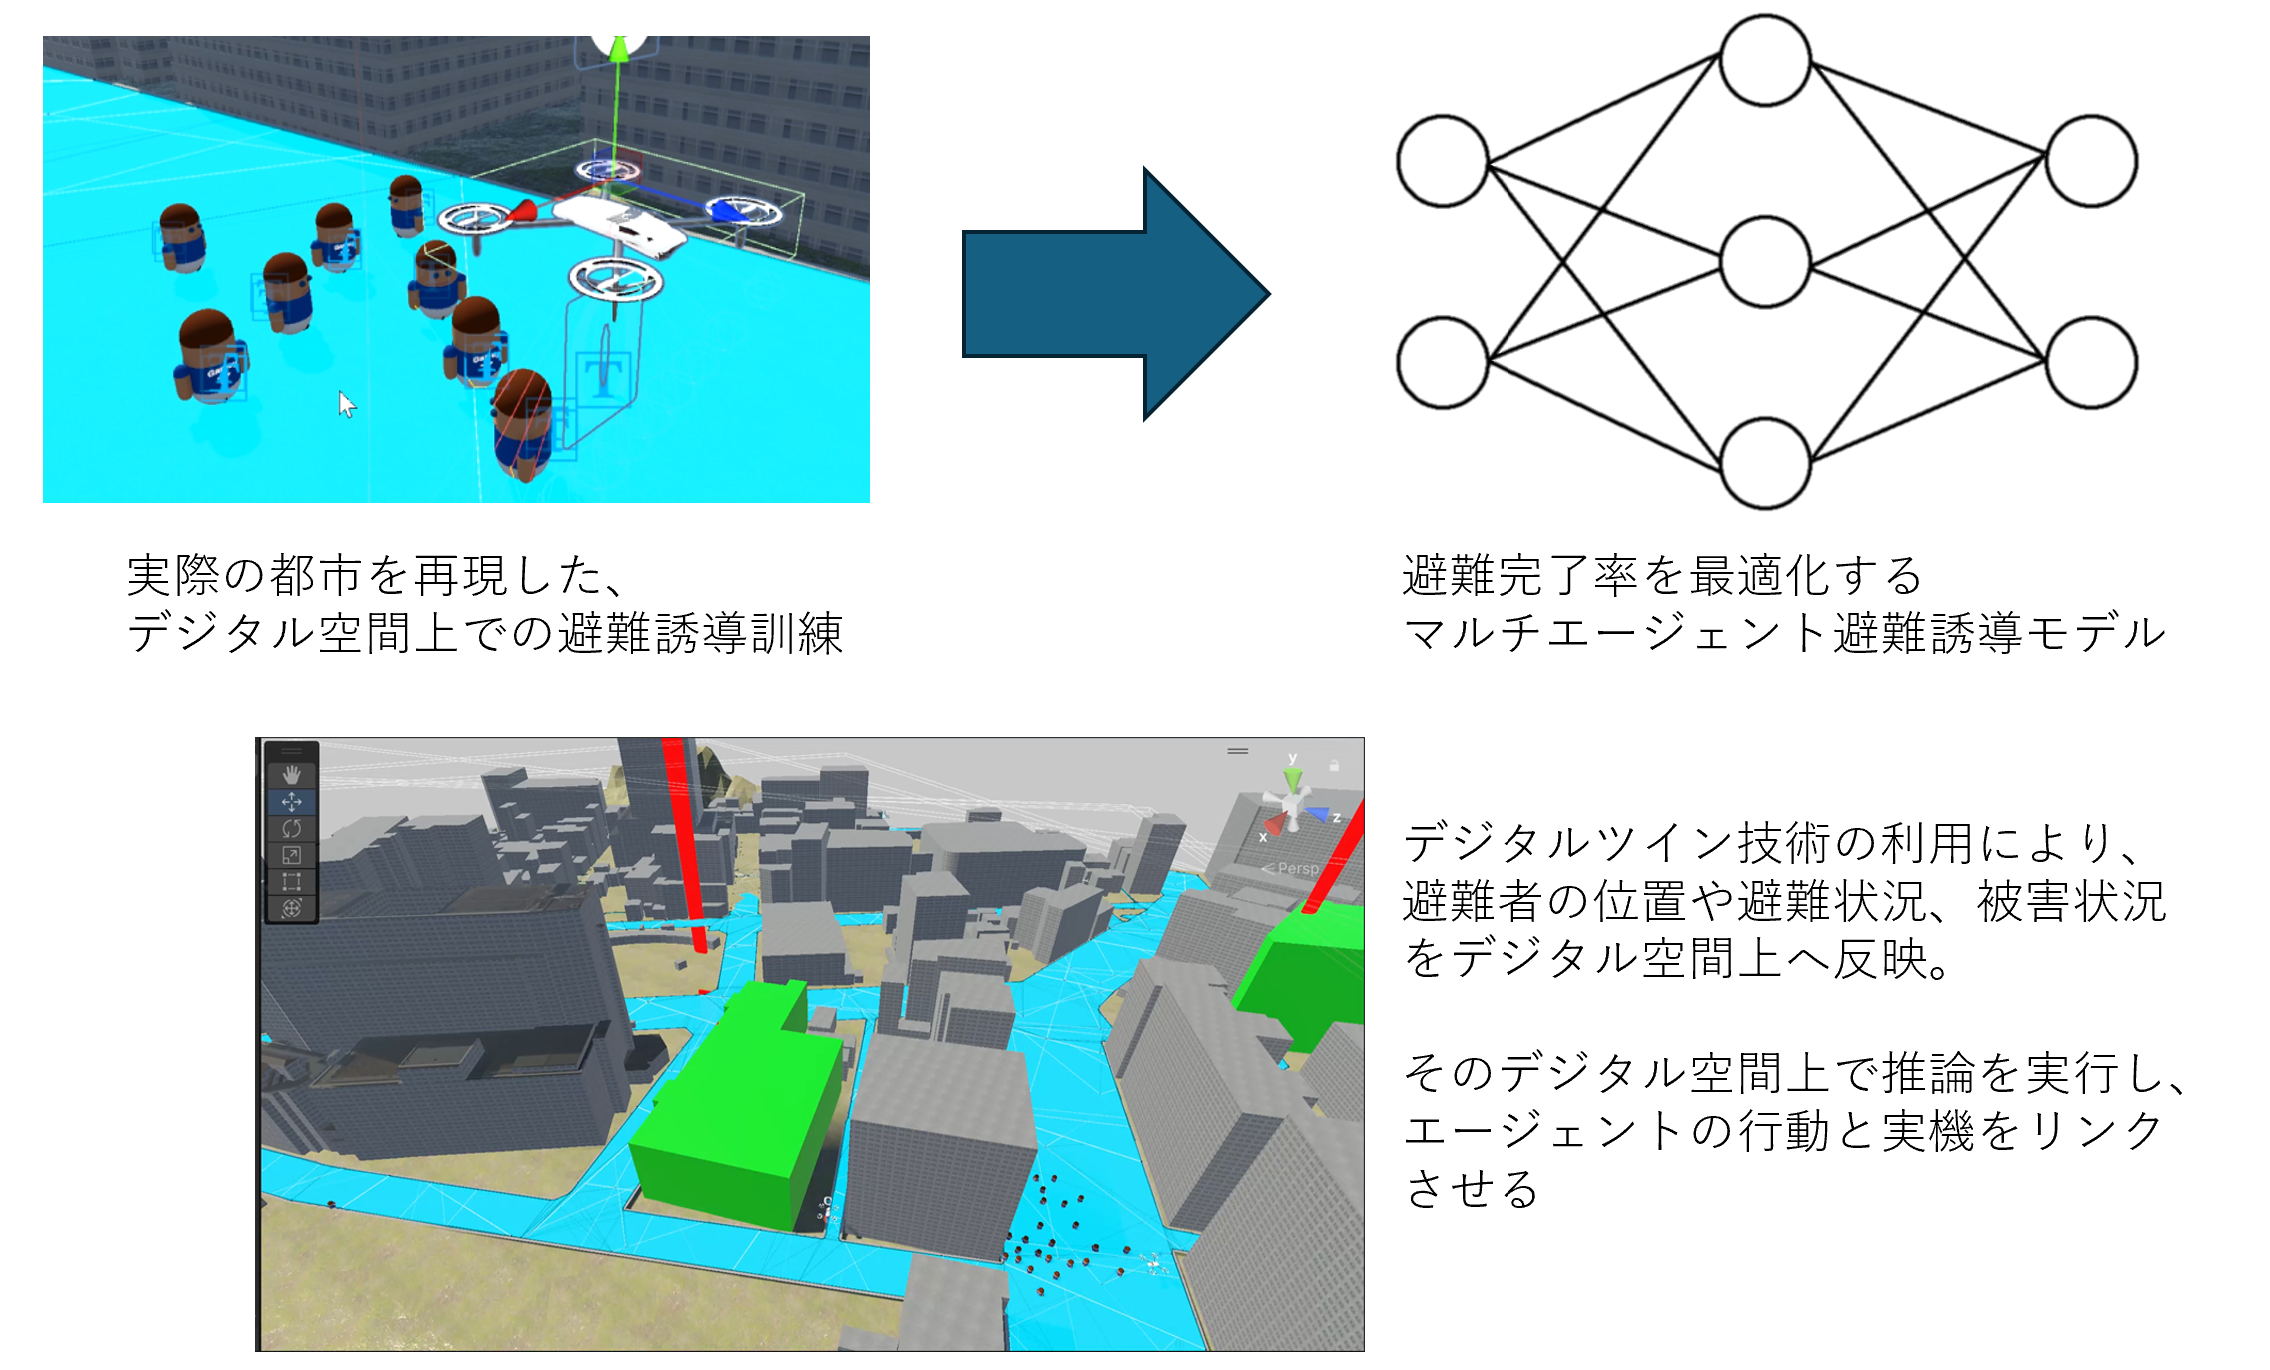
\includegraphics[width=1.0\textwidth]{Figures/2024-12-06 182816.png}
  \caption{提案手法 概略図} 
  \label{fig:01} 
\end{figure}

\section{既存研究との新規性}  
研究背景で述べたとおり,本研究は既存の研究といくつかの重要な相違点や新規性を有している.

まず,ドローンの防災活用はまだ研究が始まったばかりの新しい分野であり,本研究はその発展に寄与するものである.特に,複数のドローンを連携して運用するシステムに,AIや強化学習モデルを導入する点は,本研究の独自性を示す重要な要素である.

さらに,本研究では都市モデルを活用した訓練環境を構築し,デジタルツイン技術を通じて現実環境における運用を想定している.このように,現実世界での実用性を考慮した研究は,防災分野においても新しい試みである.

また,本研究は避難ビルの収容定員など,経路条件以外の要素を考慮した避難誘導モデルの作成にも取り組んでいる.
従来の研究の多くが,避難者自身の行動最適化を通じて避難完了率の向上を目指しているのに対し,本研究では避難完了率を最適化できる避難誘導方策そのものを追求している点で特徴的である.

以上のような取り組みにより,本研究は現実世界での応用可能性を持つ動的な津波避難誘導システムの実現を目指している.

\section{実験概要}
本研究では,津波避難誘導問題を解決するために,マルチエージェント強化学習を用いたドローン避難誘導システムを提案する.
本研究では,この問題を\textbf{1.避難者探索タスク}と\textbf{2.避難所誘導タスク}の2つの課題に分け,それぞれのタスクを解決するためのエージェントモデルをUnity上のシミュレーションにより構築する.
エージェントの訓練環境は実際の道路状況や避難所配置に限りなく近づけるため,都市モデルを活用したデジタルツイン環境を利用する.その後訓練済みエージェントモデルを利用した場合とルールベースで行動するエージェントを利用した場合それぞれのタスク遂行能力を評価するため,同一環境で比較シミュレーション実験を行う.
なお,2.避難所誘導タスクにおいては,ドローンエージェントの誘導がない場合,つまり避難者のみで避難行動を行う場合との比較も行う.
その実験結果から,最終的な避難完了率の推移や経過時間などの指標を用いて,提案手法の効果検証と実現可能性を評価する.

%TODO: 実験のイメージ図を追加
\section{シミュレーション前提条件}
\subsection{都市モデルの選定と避難所の配置条件}
環境としては,下記3つの都市の都市モデルをPLATEAU SDK for Unity\footnote{
  PLATEAU:プラトーは,国土交通省が主導する日本全国の3D都市モデルの設備・オープンデータ化プロジェクト
}
を使い3D空間上に実際の都市環境に近いシミュレーション環境を再現する.
なお,都市の選定基準については,\ref{sec:sug}章にて述べた想定場面を考慮するため下記の選定基準をもって決定した.
\begin{itemize}
  \item 南海トラフ等で津波被害が想定されている沿岸地域であること
  \item 自治体の津波避難のハザードマップが参照可能であること
  \item 地元住民以外にも多数の観光客が見込まれる,比較的規模の大きな地域であること
  \item 津波避難ビルあるいは津波避難タワーが整備されている地域であること
\end{itemize}
以上の条件を元に,下記2つの都市をモデル都市として選択した.
\begin{enumerate}
  \item 神奈川県横須賀市 市役所本庁舎 周辺沿岸地域
  \item 静岡県沼津市 沼津港周辺の一部地域
\end{enumerate}
都市モデルと実際の避難ビル(避難タワー)との位置付けは,自治体公表のハザードマップ\cite{yokosukaHazardMap}\cite{numazuHazardMap}より確認し,都市モデル上で指定した.
各モデル都市におけるシミュレーション対象範囲は以下地図\ref{fig:YokosukaMapRange}と地図\ref{fig:NumazuMapRange}の赤枠で示した範囲とする.
\begin{figure}[H]
  \centering
  % 左側の画像
  \begin{minipage}{0.45\textwidth}
      \centering
      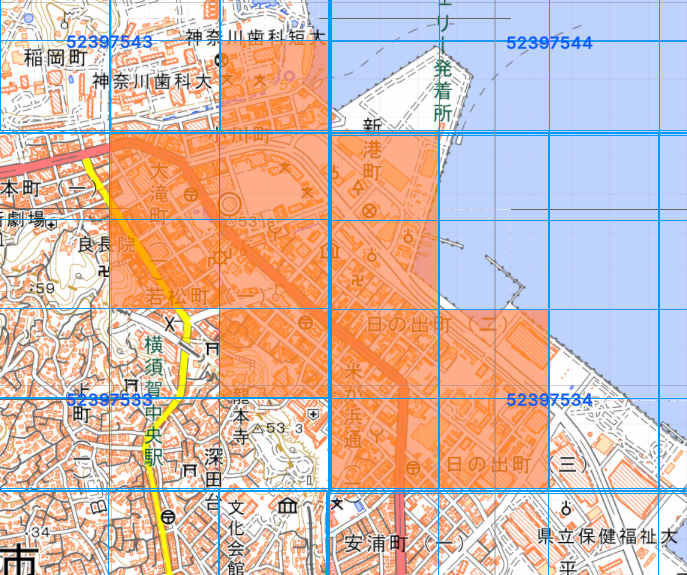
\includegraphics[width=\textwidth]{Figures/YokosukaMapRange.png} 
      \caption{横須賀市でのシミュレーション範囲}
      \label{fig:YokosukaMapRange}
  \end{minipage}
  \hfill % 隙間を調整
  % 右側の画像
  \begin{minipage}{0.45\textwidth}
      \centering
      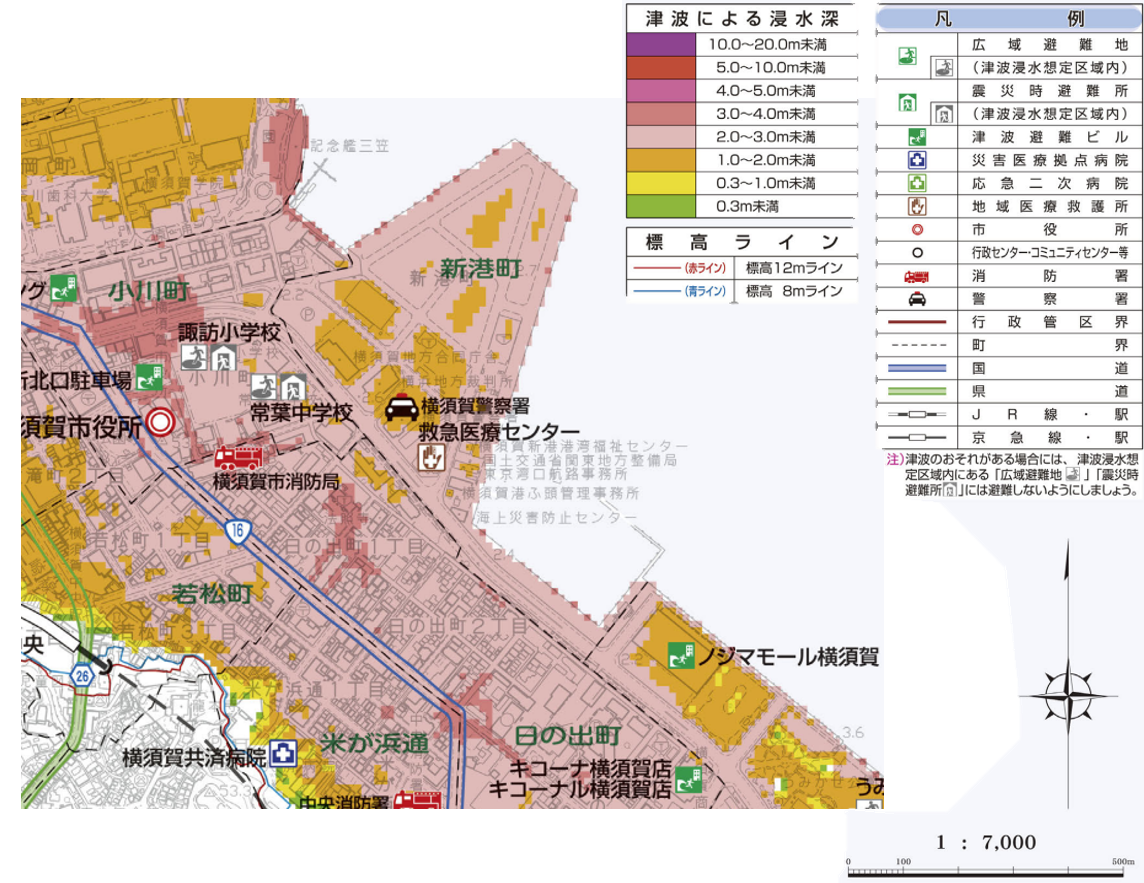
\includegraphics[width=\textwidth]{Figures/YokosukaHzaerd.png} 
      \caption{対象範囲の横須賀市のハザードマップ}
      \label{fig:right_image}
  \end{minipage}
  \label{fig:MapRange}
\end{figure}
\begin{figure}[H]
  \centering
  % 左側の画像
  \begin{minipage}{0.45\textwidth}
      \centering
      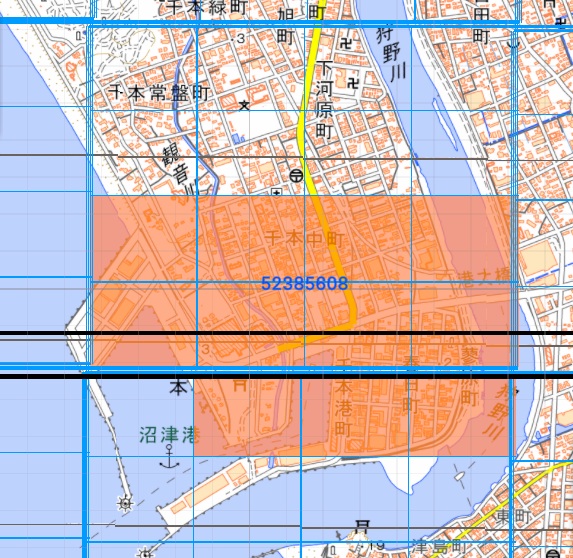
\includegraphics[width=\textwidth]{Figures/NumazuRange.png} 
      \caption{沼津市でのシミュレーション範囲}
      \label{fig:NumazuMapRange}
  \end{minipage}
  \hfill % 隙間を調整
  % 右側の画像
  \begin{minipage}{0.45\textwidth}
      \centering
      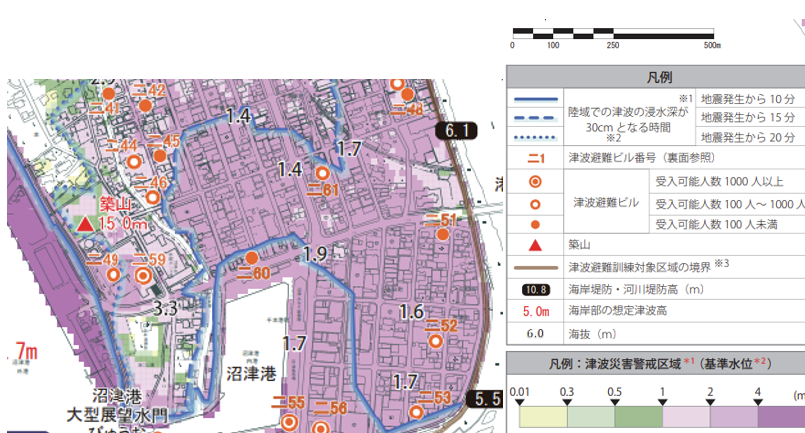
\includegraphics[width=\textwidth]{Figures/NumazuHazerd.png} 
      \caption{対象範囲の沼津市ハザードマップ}
      \label{fig:right_image}
  \end{minipage}
\end{figure}

\begin{figure}[H] 
  \centering 
  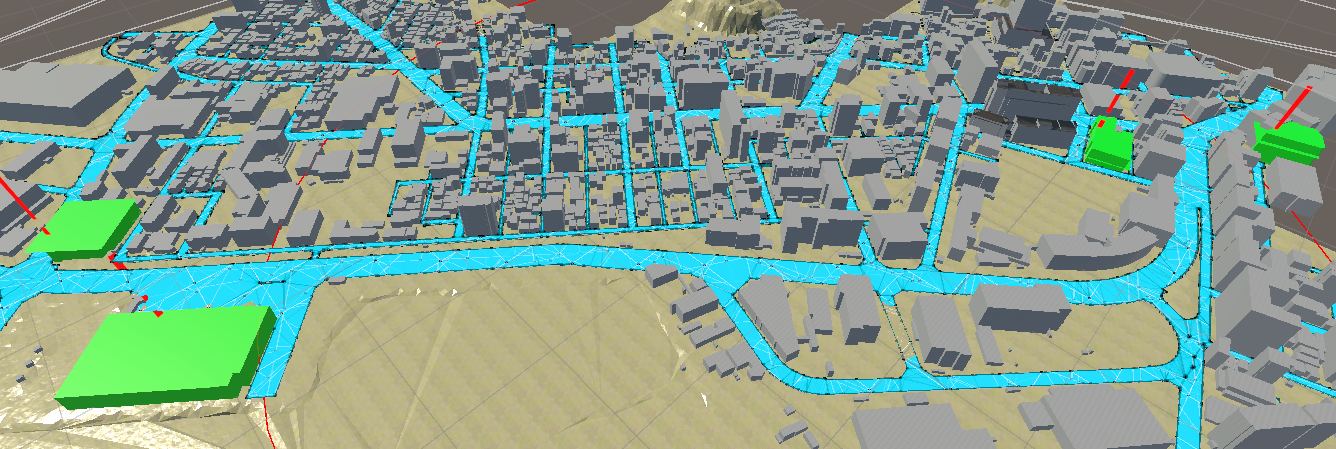
\includegraphics[width=1.0\textwidth]{Figures/2025-01-10 025916.png}
  \caption{構築したシミュレーション環境の例} 
  \label{fig:01} 
\end{figure}
なお,環境の制限時間は,内閣府が公表している南海トラフ巨大地震における各地域の津波到達予想時間のデータ\cite{dataNankaiTunamiTime}を参考に下記の範囲内でエピソード毎にランダムに決定されるものとする.
\subsection{避難者の前提条件}
避難者の初期出現位置は環境内の道路上にランダムに配置するものとする.避難者の移動方法は内閣府が公表している津波避難ガイドライン基づき徒歩移動ないしは自転車による移動を想定する.
そのため避難者の移動速度は,1m/sから3.4m/sの範囲内でランダムに設定する.
移動経路については,ナビゲーションメッシュにより指定位置までの道路上における最短経路を計算し,各避難者はその経路に従って移動するものとする.
環境内に出現する避難者の総数は予め固定するものとし,今回の実験では200名前後とした.
\subsection{避難所収容人数の前提条件}
避難誘導のタスク実験で扱う,各避難所の収容人数については,出現させる避難者が全て収容できるように避難所毎に均等に設定するものとする.
これは,第2章でも述べた収容定員を超過し,適切な避難が行えない可能性があることを考慮し,1つの避難所に大量の避難者が殺到しても,避難完了とするのを避けるためである.
また,後述するエージェントが誘導先の避難所を決定するに当たり,自身の誘導人数と避難所の収容人数を考慮させるためである.
\begin{table}[H]
  \begin{tabular}{|l|l|l|l|l|}
  \hline
       & 制限時間(秒)   & エージェント数 & 避難所数(設定収容人数) & 出現避難者総数 \\ \hline
  横須賀市 & 1800~2400 & 4       & 4棟 (50人/1棟)    & 200     \\ \hline
  沼津市  & 240~1800  & 16      & 16棟 (13人/1棟)   & 208     \\ \hline
  \end{tabular}
  \caption{各シミュレーション環境の前提条件}
\end{table}

\subsection{エージェントの前提条件}
エージェントの訓練および,マルチエージェントモデルの作成は,都市ごとに避難所の配置分布や道路状態といった環境条件が異なるため,各都市ごとに行うものとする.
シミュレーションにおいて,エージェントの初期位置は,避難者の初期位置と同様に環境内の道路上にランダムに配置するものとする.
なお,出現するエージェントの数は,環境内の避難所1つあたりにつき1機とする.
移動方法の詳細は後述する各実験の章にて述べる.エージェントは自身の移動が完了するごとに決定を要求し,環境の観測を行った後,行動を決定する.
なお,強化学習アルゴリズムにはMA-POCAを利用する.


\section{避難者探索タスク実験方法}
この実験ではエージェントは環境内の避難者を探索し,制限時間以内にできるだけ多くの避難者を見つけるタスクを行う.
エピソード開始時,エージェントは環境内のランダムな道路上に配置される.
その後エージェントは観測として,自身の環境内に位置情報と移動速度,現在発見した避難者の人数,制限時間と経過時間,他のエージェントの位置情報を取得する.
またエージェントはレイキャスト\footnote{レイキャスト(Raycast)は,コンピュータグラフィックスや物理エンジンで使用される技術であり,特定の方向に仮想的な「線(レイ)」を発射して,それがどのオブジェクトに当たるかを検出する手法.検知対象オブジェクトの位置情報を取得できる.}観測により,自身の付近に避難者がいる場合,その避難者の位置情報を観測することができる.
その後,エージェントは行動として,自身の移動速度を\SI{1.0}{\meter\per\second}から\SI{2.0}{\meter\per\second}の間で移動速度を出力する.また,現在位置からの移動量を半径\SI{50}{\meter}以内の範囲で決定し,移動を開始する.
避難者は半径\SI{60.0}{\meter}以内でエージェントを視認できる場合,そのエージェントを追従し,エージェントの報酬として$\frac{1}{避難者の総数}$の正の報酬を得る.
制限時間を超えるか全ての避難者が発見された時点でシミュレーションのエピドートは終了する.
\begin{figure}[H] 
  \centering 
  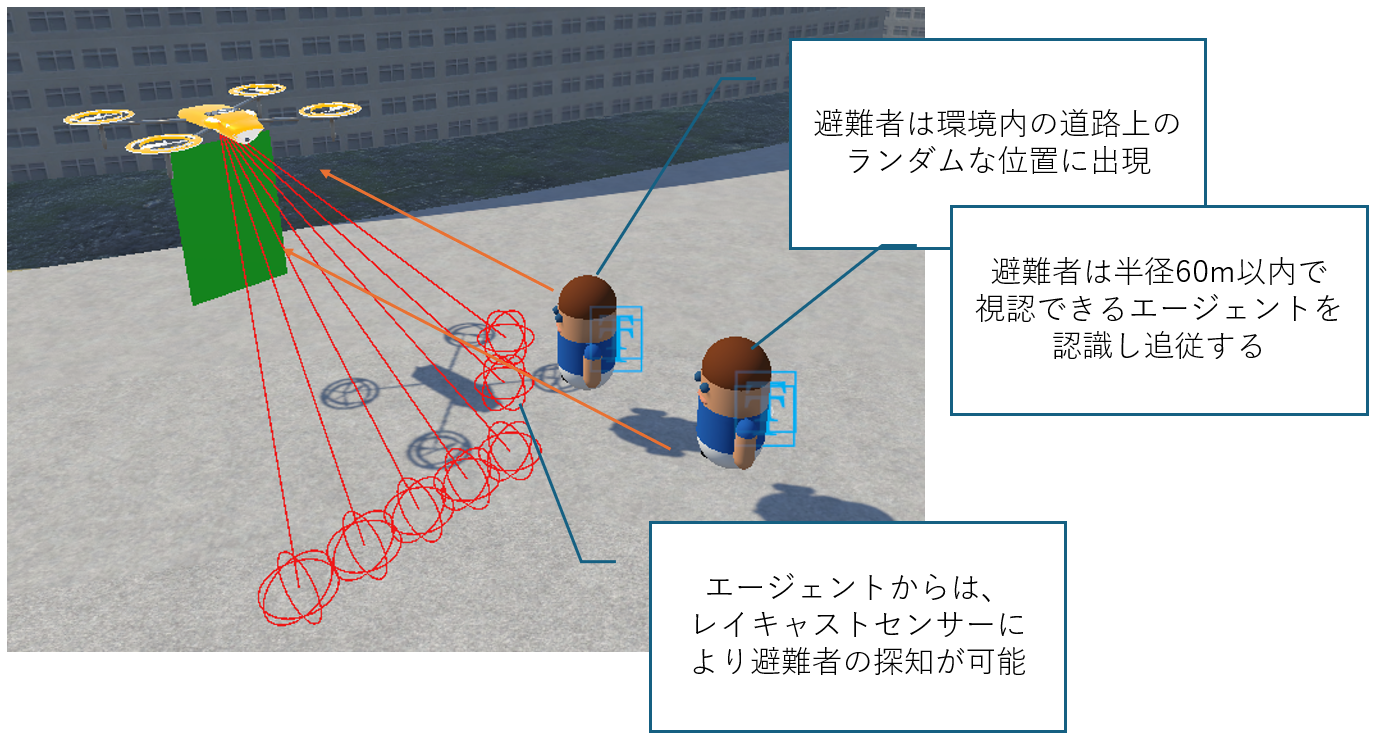
\includegraphics[width=1.0\textwidth]{Figures/SearchEx.png}
  \caption{避難者探索タスクのイメージ図} 
  \label{fig:01} 
\end{figure}
\paragraph{エージェントの観測}
エージェントは環境内の以下の情報を観測することができる.
\begin{itemize}
  \item 自身の位置情報(X,Y,Z座標)
  \item 自身の移動速度(浮動小数値)
  \item 現在発見した避難者の人数
  \item 現在追従している避難者の平均移動速度
  \item 制限時間と経過時間
  \item 他のエージェントの情報
  \begin{itemize}
    \item 他のエージェントの位置情報(X,Y,Z座標)
    \item 他のエージェントが発見した避難者の人数
  \end{itemize} 
\end{itemize}

\paragraph{エージェントの行動}
エージェントは観測情報に基づいて以下の行動を連続値として取ることができる.
\begin{itemize}
  \item 移動速度(\SI{1.0}{\meter\per\second}から\SI{2.0}{\meter\per\second}の間での連続値)
  \item 現在位置からの移動量(半径\SI{50}{\meter}以内の範囲での連続値)
\end{itemize}
なお,エージェントが行動として出力した移動量に基づき,移動先の座標を決定するが,移動先の座標はナビゲーションメッシュ上の道路上に限定するものとするため,
計算した移動先の座標がナビゲーションメッシュ上にない場合は最寄りのナビゲーションメッシュ上の座標位置に移動するものとする.

\paragraph{エージェントの報酬}
各エージェントは発見した避難者の人数に応じて$\frac{1}{避難者の総数}$の正の個別報酬を得る.
また,同時にグループ報酬として,$\frac{1}{避難者の総数}$の正の報酬を得る.

\paragraph{評価と比較}
この実験では,マルチエージェント強化学習を用いたエージェントモデルとルールベースで行動するエージェントモデルの2つの行動パターンを比較する.
ルールベースで行動するエージェントモデルは,ランダムに移動速度と移動量を決定し,避難者を探索するものとする.
以上の2つの行動パターンにおいて,最終的な避難者の発見率とその推移などの指標を用いて,マルチエージェントモデルとルールベースモデルの有効性を評価する.

\section{避難所誘導タスク実験方法}
この実験ではエージェントは事前に割り当てられた避難者グループを指定された避難所まで誘導するタスクを行う.
エピドート開始時,エージェントは環境内のランダムな道路上に配置される.そのエージェントの周辺に10人から40人の避難者がランダムな人数配置される.
次にエージェントは観測として自身の環境内での位置情報や割り当てられている避難者の人数,各避難所までの移動距離や収容人数などの情報を取得する.その観測に基づいてエージェントは行動として,自身の移動速度を$1.0m/s$から$3.0m/s$の間で,誘導先である避難所を1つ決定し移動することができる.
環境内の各避難所には収容可能人数が設定されており,避難者が避難所に到達するとその避難所の収容可能人数が減少する.
避難者はエージェントに追従し,避難所に到達すると避難者は避難所に収容される.なお,避難所に収容される避難者の数は避難所の収容人数を超えることはないものとする.
もし,避難時点でその避難所の収容定員を超える場合,避難者はエージェントに追従し続け,次のエージェントの行動決定まで待機する.
制限時間を超えるか全ての避難者が避難所に収容された時にシミュレーションのエピソードは終了する.
\begin{figure}[H] 
  \centering 
  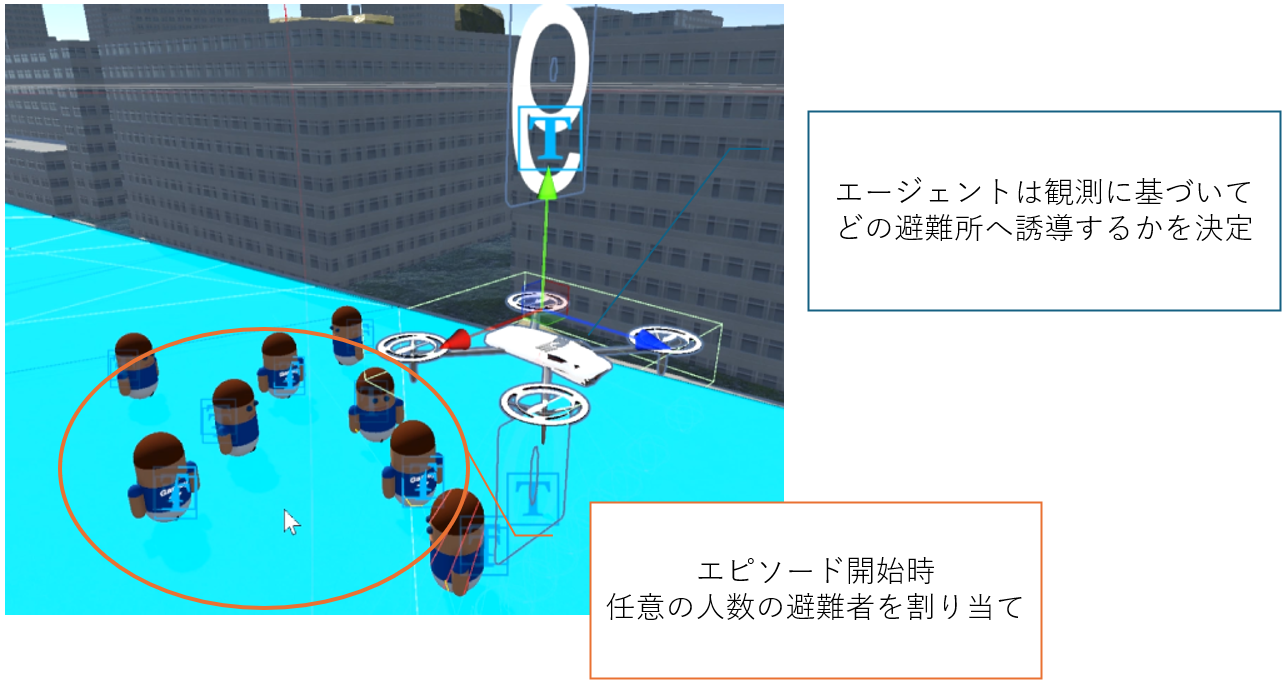
\includegraphics[width=1.0\textwidth]{Figures/GuidTaskEx.png}
  \caption{避難所誘導タスクのイメージ図}
  \label{fig:01} 
\end{figure}
\paragraph{エージェントの観測}
エージェントは環境内の以下の情報を観測することができる.
\begin{itemize}
  \item 自身の位置情報(X,Y,Z座標)
  \item 自身の移動速度(浮動小数値)
  \item 割り当てられている避難者の人数
  \item 避難者グループの平均移動速度
  \item 各避難所の位置情報(X,Y,Z座標)
  \item 各避難所までの移動距離
  \item 各避難所の現在の収容可能人数
  \item 他のエージェントの情報
  \begin{itemize}
    \item 他のエージェントの位置情報(X,Y,Z座標)
    \item 他のエージェントが移動する避難所の位置情報(X,Y,Z座標)
    \item 他のエージェントが誘導している避難者の人数
  \end{itemize}
\end{itemize}
  
 
\paragraph{エージェントの行動}
エージェントは観測情報に基づいて以下の行動を取ることができる.
\begin{itemize}
  \item 移動先の避難所
  \item 自身の移動速度
\end{itemize}

\paragraph{エージェントの報酬}
各エージェントは誘導した避難所に自身に割り当てられている避難者が到達するとその人数に応じて$+1$の正の個別報酬を得る.
また,グループ報酬として,シミュレーション終了時点での最終的な避難完了率を計算し,その値に応じて$0$~$1$の正のグループ報酬を得る.

\paragraph{評価と比較}
この実験では,マルチエージェント強化学習を用いたエージェントモデルとルールベースで行動するエージェントモデル,避難者単独行動のパターンの3つの行動パターンを比較する.
ルールベースで行動するエージェントモデルは,自身から最も近い受け入れ可能な避難所までの最短経路を計算し,避難所に到達するまでの移動速度を一定に設定するものとする.
避難者単独のパターンでは,各避難者は自身から最寄りの避難所までの最短経路を計算し,その経路に従って移動するものとする.
なおこの時避難者は,移動先の避難所の収容人数を知ることはできず,避難所に到達した段階で収容可能人数を超える場合,次の最寄りの避難所に向かうものとする.\par

以上の3つの行動パターンにおいて,最終的な避難完了率,経過時間ごとの避難完了率の推移,の指標を用いて,マルチエージェントモデルの有効性を評価する.

\chapter{実験結果と考察}
本章では、沿岸地域における津波避難誘導をドローンエージェントに行わせる事を考え
\section{避難者探索タスク実験}

\section{避難所誘導タスク実験}
\chapter{結論}
本章では、本研究で提案したマルチエージェントドローンによる津波避難誘導システムの実現可能性について、実験結果および我が国における災害対策の現状を踏まえてまとめる。また、本研究の成果を基にした今後の展望についても述べる。

\section{実験のまとめ}
本研究は、マルチエージェント強化学習を用いたドローンによる津波避難誘導システムを提案し、その効果を3D都市モデルを活用したシミュレーション実験で検証した。
実験では,津波避難誘導のタスクを\textbf{1.避難者探索と収集}と\textbf{2.避難者群衆の誘導}.の2つのタスクに置けるマルチエージェントモデルを作成しその効果を検証した.
その結果から、以下の点が明らかとなった。

%TODO: 実験結果からルールベースでのドローンエージェントが有効であることを述べる
\paragraph{ルールベースでのドローンエージェントの有効性}
まず、ルールベースでのドローンエージェントが避難者の探索および誘導において一定の有効性を示した点である。
避難者探索のタスクにおいては,都市の道路状況やエージェントの初期位置,エージェントの機数により結果に変動はあるが,
ランダムに行動するドローンエージェントの場合でも比較的短時間で35\%から最大で80\%程度の避難者を発見,エージェントの各個において誘導すべき群衆を形成することができた.
また,群衆の避難所誘導タスクにおいては,避難所までの最短経路を進む避難者のみで行動するケースよりも,ルールベースでの誘導を実施する方が若干ではあるが避難完了を速く行わせることができることが確認された.

ただし,これらのシミュレーション条件にはいくつか課題が残されている.
探索モデルの場合は,避難者の出現位置の前提条件として,環境内の道路上にランダム偏りなく出現するという条件があり,実際の都市空間においては住宅街や大通りなど場所により避難者の人数分布は偏る可能性がある.
避難者の出現分布を偏らせた場合での検証が必要である.
また,避難所誘導モデルにおいては,エージェントの初期位置の違いにより,エピソード毎の最終的な避難完了率にバラつきがある点や,避難所毎の収容人数に偏りを持たせた場合での検証が必要である.
また,避難者の人数規模についても再考が必要である.本研究ではサンプルとして200名前後での各タスク遂行実験を行ったが,実際の各都市における想定される避難者数を考慮したさらに大規模な検証が必要である.

\paragraph{マルチエージェントモデルの課題}
%TODO: マルチエージェントモデルが上手くいななかった理由を述べる→改善点の提案
本研究では,探索と誘導どちらのタスクにおいても,今回作成したマルチエージェントモデルはルールベースでの性能には及ばなかった.
これは,モデルの学習が全体として上手くいかず,エージェントが適切な協調行動を行う方策を学習できなかったためである.
学習が上手くいかなかった要因としては複数考えられるが,モデルの学習過程を分析すると次の様なことが考えられる.
探索タスクにおいては,累積報酬が学習過程で増加せず,最終的に減少傾向にあった点と価値関数の平均損失が学習過程で減少している点が確認された.
また,誘導タスクにおいては、累積報酬は沼津市のケースでは若干の増加傾向を示したものの横須賀市のケースでは学習過程全体で減少傾向を示した.また全体として,価値関数の平均損失の値が大きく,モデルの予測性能が低いことが伺える.
このことから,エージェントが訓練課程で誤った方策を学習してしまった可能性が高く、最終的な結果が良くならなかったものと推察される.

\section{ドローンによる津波避難誘導の実現可能性}
%TODO: ここから現在の研究背景を元に,実現可能性について論じる.
ドローン(無人航空機)の津波避難における活用が既に我が国でも進められており一部の自治体では,運用段階に入っていることを紹介した.
また東日本大震災以後,避難誘導において避難者のみならず,誘導にあたる人員も含めた人的被害を低減することの重要性が再認識されている現状がある.
加えて,新型コロナウイルスによる政府の自粛要請も終わり,観光客数が再び増加傾向にある中,
土地勘のない大勢の観光客も含めた避難者の津波避難行動については,津波避難ビルの配置や収容定員超過等の理由により,現状では十分な避難対策が行われているとは言い難い状況が先行研究で示された.
このような状況において,津波避難誘導の一連のオペレーションをドローンによって代替することは,人的被害を低減する観点からも有効であると考えられる.
本研究における実験結果が示すように,マルチエージェントニューラルネットワークモデルを用いたドローンの避難誘導には課題が残されているが,
ルールベースでのドローンエージェントによる避難誘導は一定の効果が期待でき,先行研究事例も含め,津波避難誘導をドローンで代替できる可能性とその有効性を確認することができた.
\section{今後の展望}
本研究の結果を踏まえ、以下の方向性でさらなる発展が期待される。

まず、報酬設計の見直しが必要である。具体的には、避難者を発見した際の報酬だけでなく、未探索エリアの探索や協調行動に基づく報酬を導入することで、エージェントの探索効率を向上させることが可能である。また、エントロピーの制御を通じて、行動方針の収束を促進しながら適切な探索と利用のバランスを取る仕組みを設ける必要がある。

次に、シミュレーション環境をさらに現実に近づけることも重要である。本研究で構築した環境は、現実の地形や避難所配置を模倣したものであるが、気象条件やリアルタイムの人口動態データを取り入れることで、より現実的なシナリオでの検証が可能となるであろう。

さらに、実環境における検証も進めるべきである。例えば、自治体や研究機関と連携し、災害対応訓練の一環として提案システムを試験運用することで、その有効性を実証し、改良を行うことができる。また、複数ドローンのリアルタイム制御や通信の安定性を向上させるための技術的な工夫も求められる。

最終的に、本研究の成果は、津波避難誘導に限らず、風水害や地震など、様々な災害シナリオへの応用が期待される。マルチエージェント強化学習と自律型ドローンの組み合わせは、防災技術の新たな可能性を広げるものであり、今後の防災分野におけるさらなる研究と実用化が待たれる。

\chapter{結論}


% ===謝辞(任意)===
% \chapter*{謝辞}

まず,研究室で2年間,研究テーマ相談から,実験内容の決定,論文の着地点の相談まで,
実に多方面で終始多大なご指導を賜った三宅陽一郎先生に深く感謝を申し上げます。
研究成果か思う様に進まない時期もありましたが,先生のご指導のおかげで,最後まで諦めずに研究を続けることができました。
また本研究以外にも,産学連携プロジェクトの監督,昨年度のオープンハウス企画のご相談などにもご協力頂きました。心より感謝いたします。ありがとうございました。

この2年間の研究室活動を通じ,単に知見と技術力を広げただけでなく,ゲームAI技術を社会課題に応用できる可能性と有意義さ,そしてなにより面白さを知ることができました。
これも,先生の研究室に所属し研究活動を行えたからこそ得られたものであると感じております。

また,リアルミーティングや自主的なゼミ,オープンハウスでの企画,外部コンペティションへの参加など,先生以外の研究室の皆様にも多大なるご協力を頂きました。
また,日ごろの研究についてもアドバイスを賜りとても助かりました。
この場を借りまして,心より感謝申し上げます。
また,研究を続けるために支援をくださった家族にも感謝いたします。

実に様々な方々に支えられ,助けられ,この論文を完成させることができました。
改めて,心より感謝申し上げます。ありがとうございました。

% ===参考文献===
\bibliography{main}
\bibliographystyle{unsrt}
    

% ===付録(任意)===
% \appendix
\chapter*{付録A}
\section{探索タスクマルチエージェントモデルの学習結果}
\subsection{横須賀市の場合}
\begin{figure}[H] 
  \centering 
  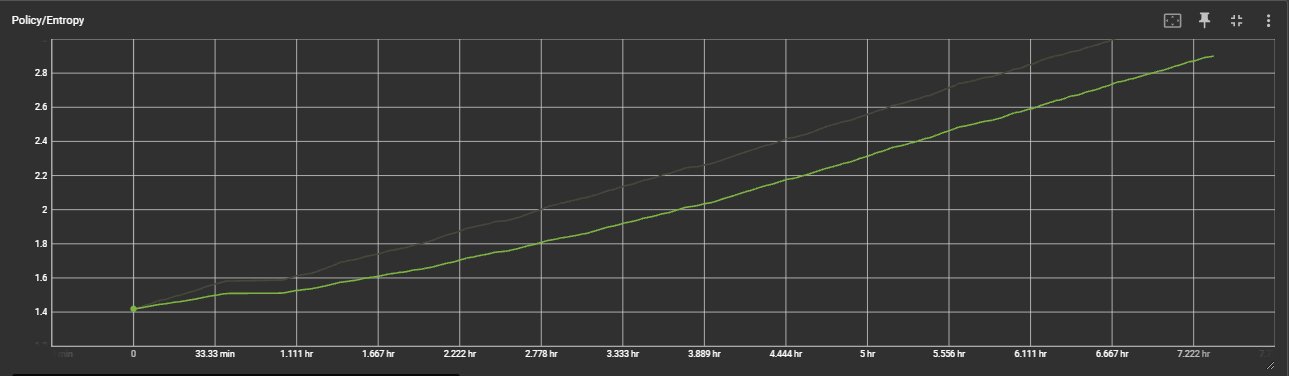
\includegraphics[width=0.8\textwidth]{Figures/App-YokosukaSearchEntropy.png}
  \caption{エントロピーの推移} 
  \label{fig:fig-01}
\end{figure}
\begin{figure}[H] 
  \centering 
  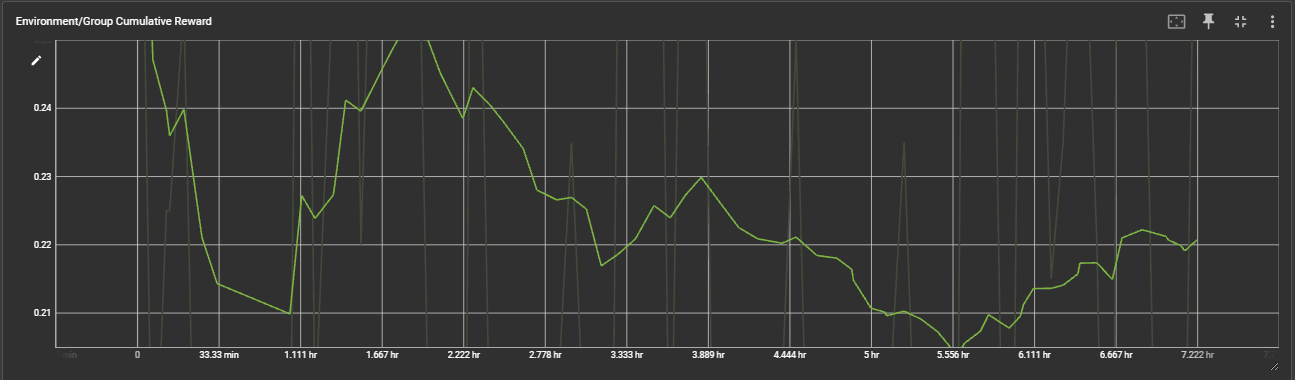
\includegraphics[width=0.8\textwidth]{Figures/App-YokosukaSearchGroupRward.png}
  \caption{グループ累積報酬の推移} 
  \label{fig:fig-01}
\end{figure}
\begin{figure}[H] 
  \centering 
  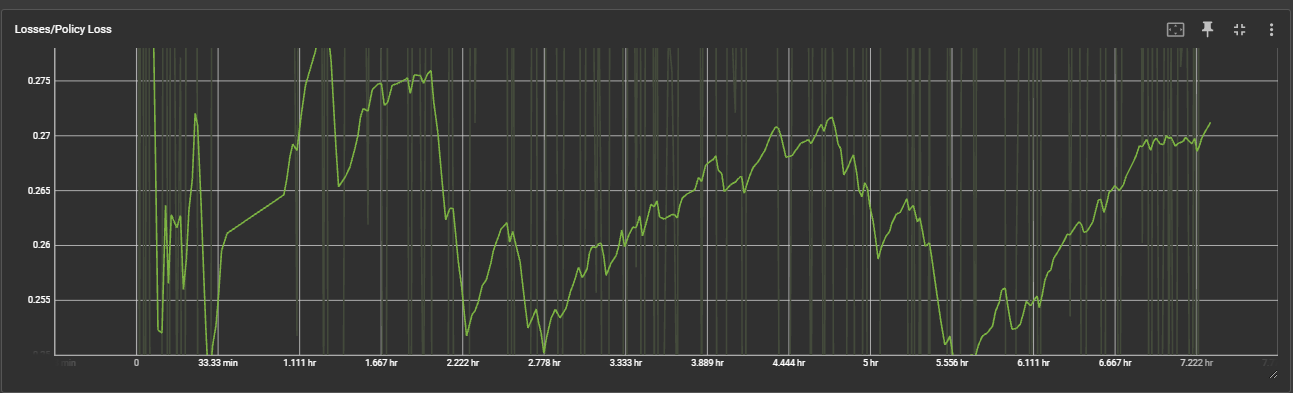
\includegraphics[width=0.8\textwidth]{Figures/YokosukaSearch-PolicyLoss.png}
  \caption{ポリシー関数の平均損失} 
  \label{fig:fig-01}
\end{figure}
\begin{figure}[H] 
  \centering 
  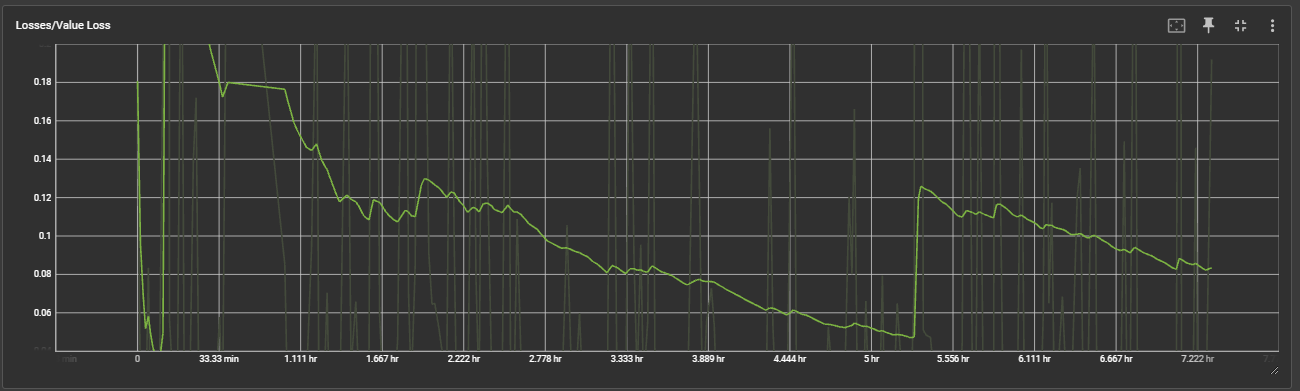
\includegraphics[width=0.8\textwidth]{Figures/App-YokosukaSearchVlueLoss.png}
  \caption{価値関数の平均損失} 
  \label{fig:fig-01}
\end{figure}


\subsection{沼津市の場合}
\begin{figure}[H] 
  \centering 
  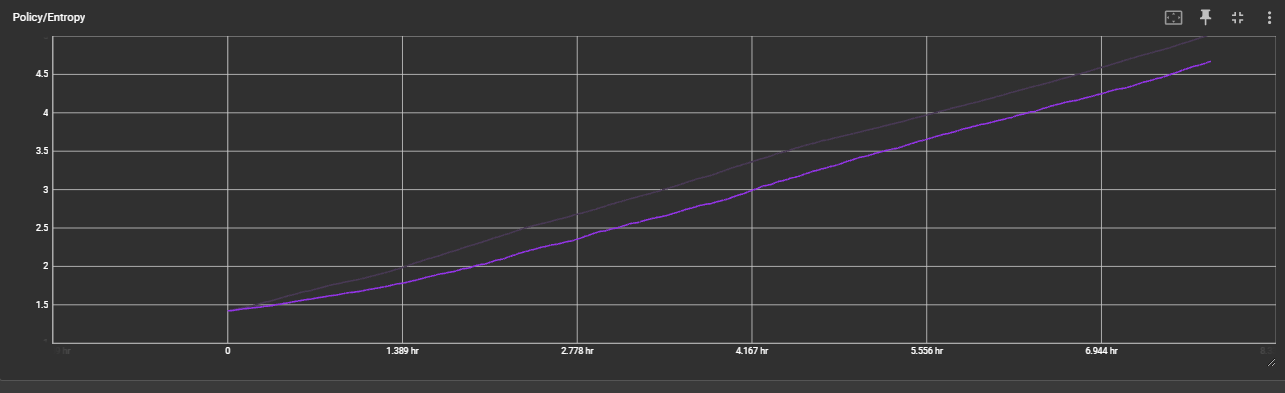
\includegraphics[width=0.8\textwidth]{Figures/NumazuSearch-Entropy.png}
  \caption{エントロピーの推移} 
  \label{fig:fig-01}
\end{figure}
\begin{figure}[H] 
  \centering 
  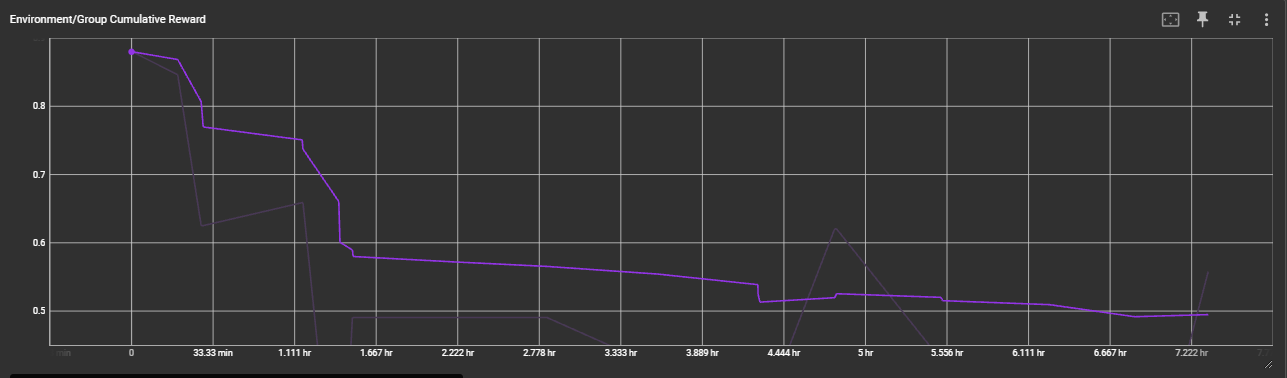
\includegraphics[width=0.8\textwidth]{Figures/NumazuSearch-GroupReward.png}
  \caption{グループ累積報酬の推移} 
  \label{fig:fig-01}
\end{figure}
\begin{figure}[H] 
  \centering 
  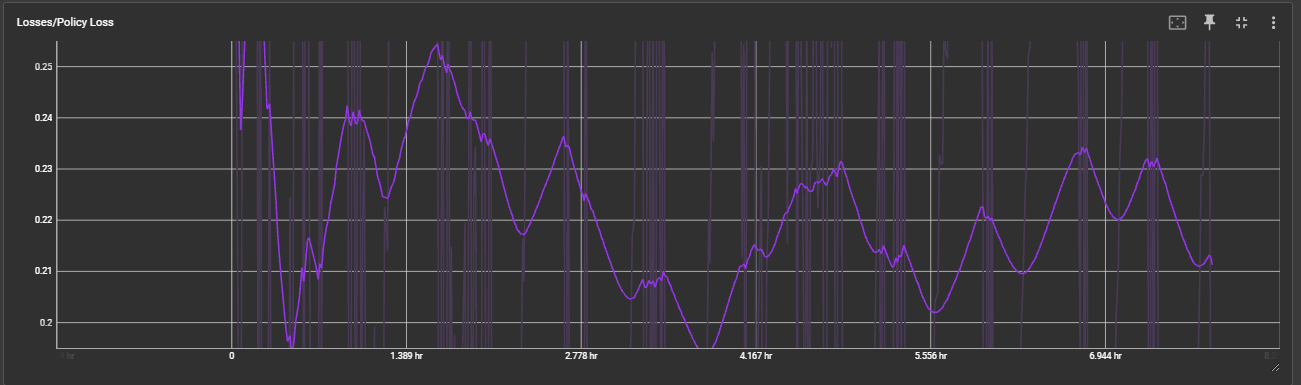
\includegraphics[width=0.8\textwidth]{Figures/NumazuSearch-PolicyLoss.png}
  \caption{ポリシー関数の平均損失} 
  \label{fig:fig-01}
\end{figure}
\begin{figure}[H] 
  \centering 
  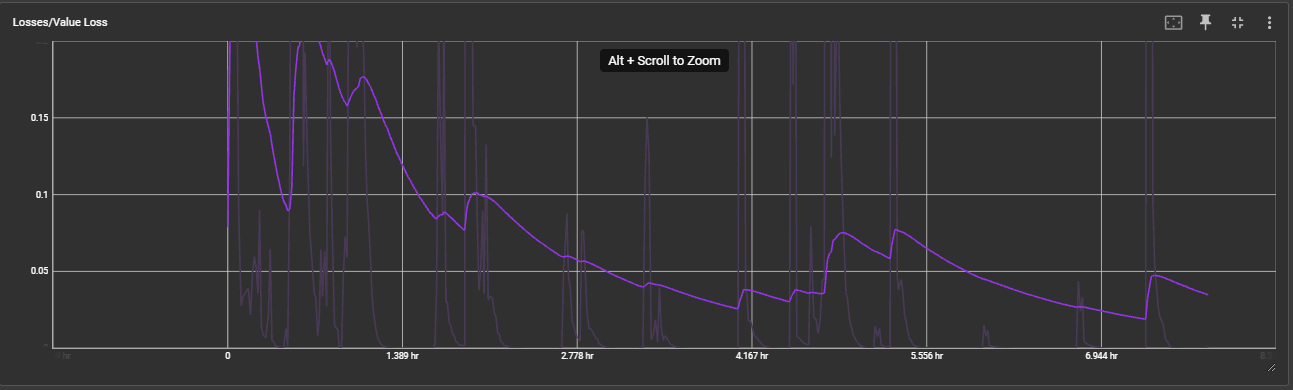
\includegraphics[width=0.8\textwidth]{Figures/NumazuSearch-ValueLoss.png}
  \caption{価値関数の平均損失} 
  \label{fig:fig-01}
\end{figure}

\section{誘導タスクマルチエージェントモデルの学習結果}

\subsection{横須賀市の場合}
\begin{figure}[H] 
  \centering 
  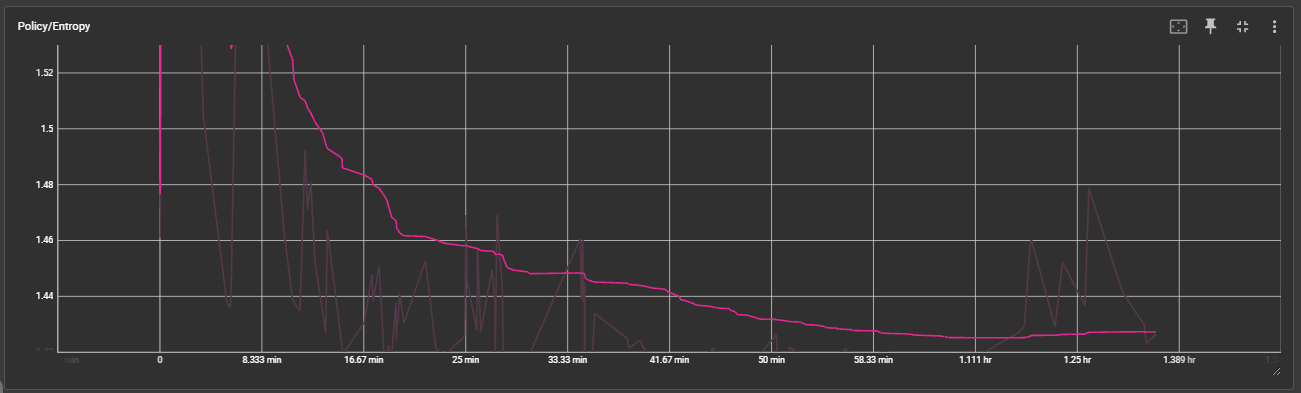
\includegraphics[width=0.8\textwidth]{Figures/Yokosuka-Entropy.png}
  \caption{エントロピーの推移} 
  \label{fig:fig-01}
\end{figure}
\begin{figure}[H] 
  \centering 
  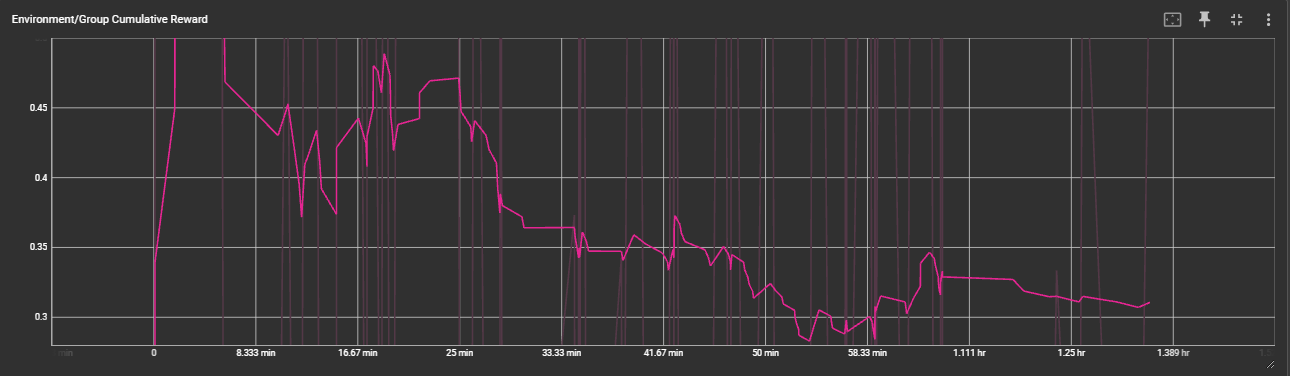
\includegraphics[width=0.8\textwidth]{Figures/Yokosuka-GroupReward.png}
  \caption{グループ累積報酬の推移} 
  \label{fig:fig-01}
\end{figure}
\begin{figure}[H] 
  \centering 
  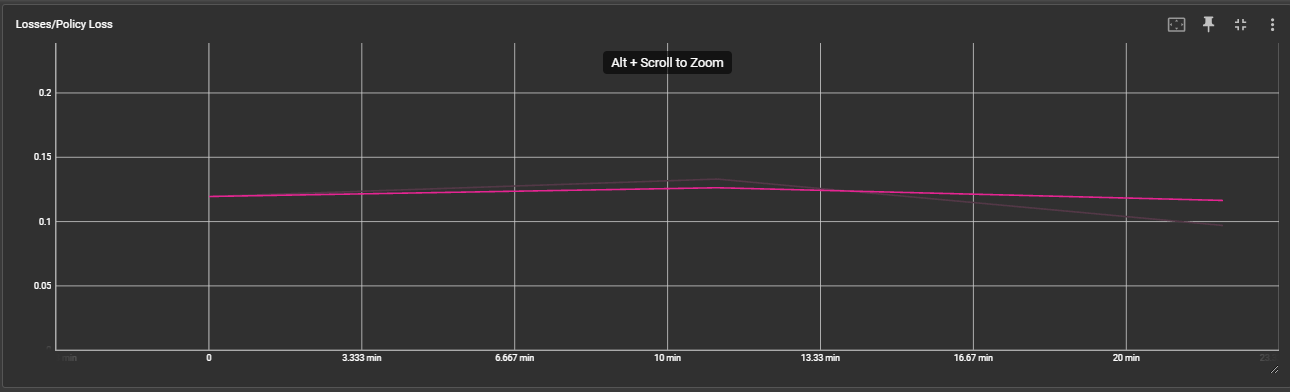
\includegraphics[width=0.8\textwidth]{Figures/Yokosuka-PolycyLoss.png}
  \caption{ポリシー関数の平均損失} 
  \label{fig:fig-01}
\end{figure}
\begin{figure}[H] 
  \centering 
  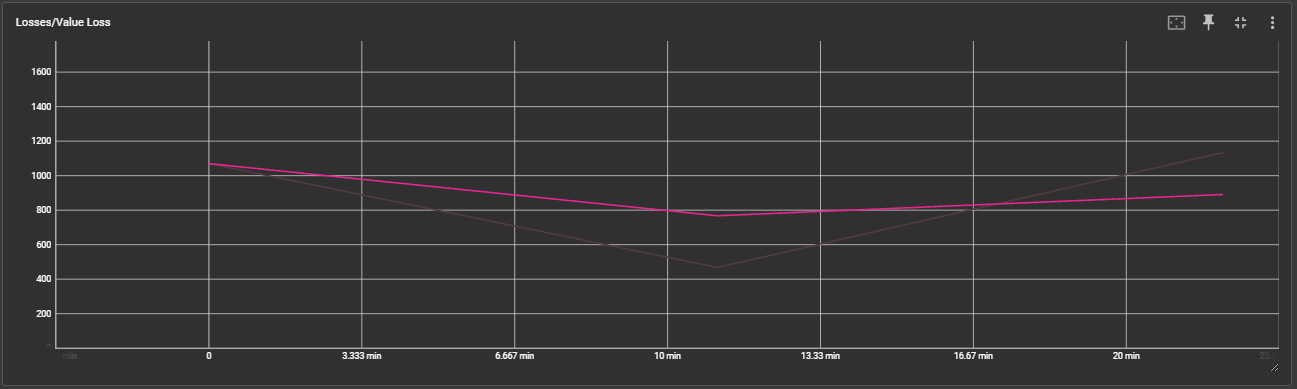
\includegraphics[width=0.8\textwidth]{Figures/YokosukaValueLoss.png}
  \caption{価値関数の平均損失} 
  \label{fig:fig-01}
\end{figure}


\subsection{沼津市の場合}
\begin{figure}[H] 
  \centering 
  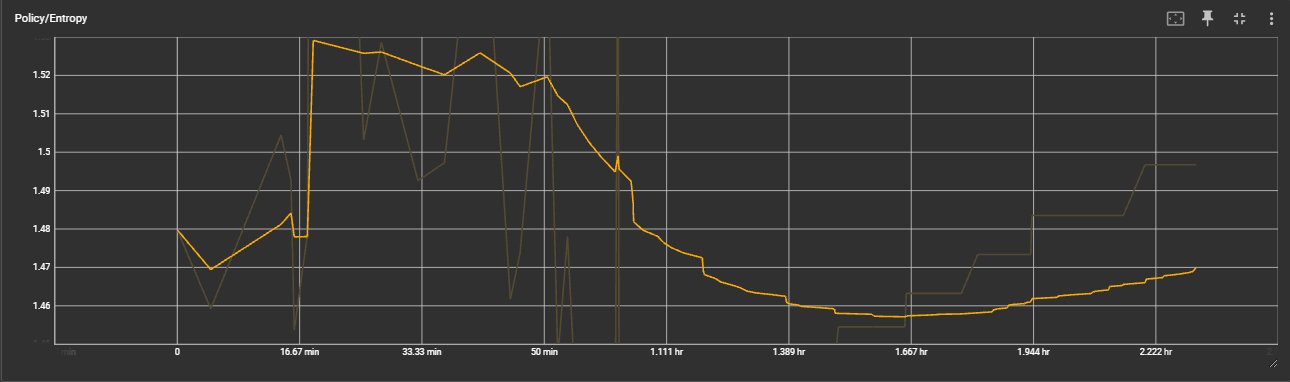
\includegraphics[width=0.8\textwidth]{Figures/NumazuEntropy.png}
  \caption{エントロピーの推移} 
  \label{fig:fig-01}
\end{figure}
\begin{figure}[H] 
  \centering 
  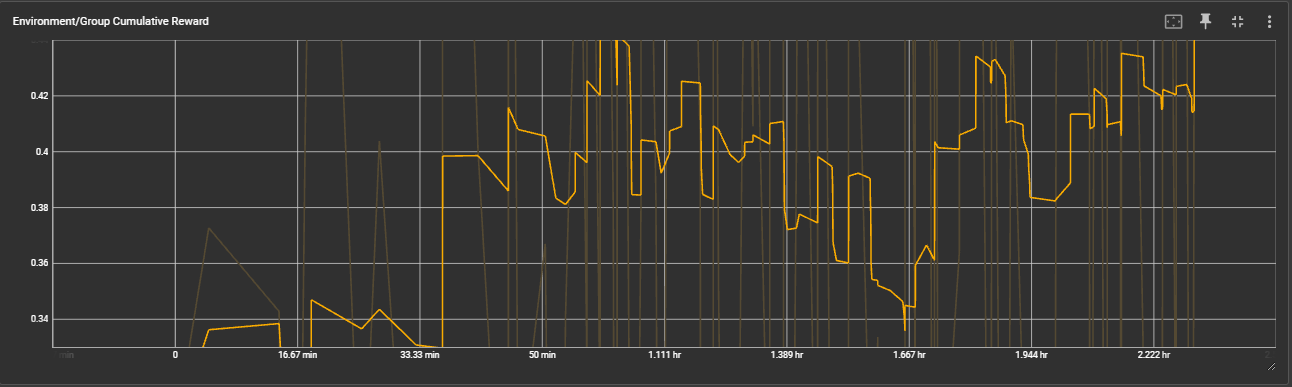
\includegraphics[width=0.8\textwidth]{Figures/NumazuGroupReward.png}
  \caption{グループ累積報酬の推移} 
  \label{fig:fig-01}
\end{figure}
\begin{figure}[H] 
  \centering 
  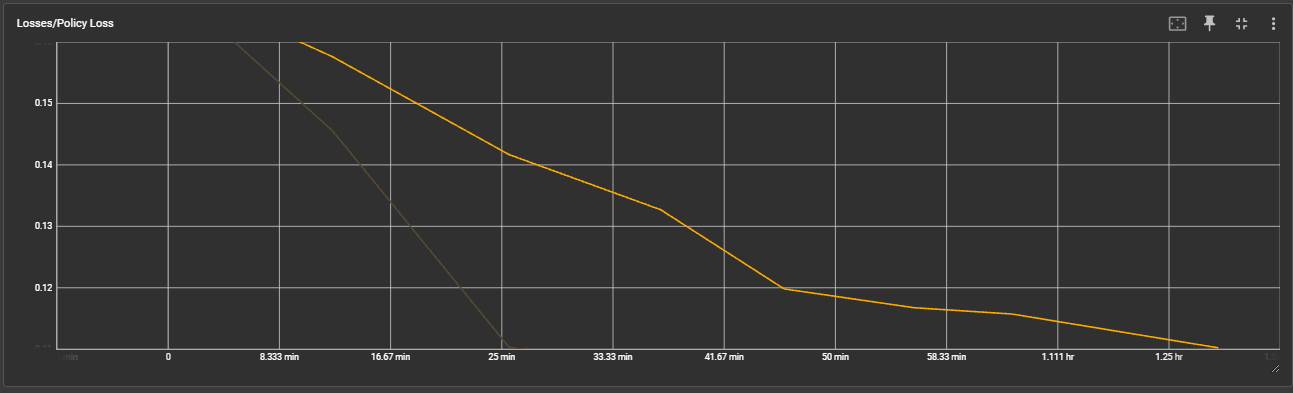
\includegraphics[width=0.8\textwidth]{Figures/NumazuPolicyLoss.png}
  \caption{ポリシー関数の平均損失} 
  \label{fig:fig-01}
\end{figure}
\begin{figure}[H] 
  \centering 
  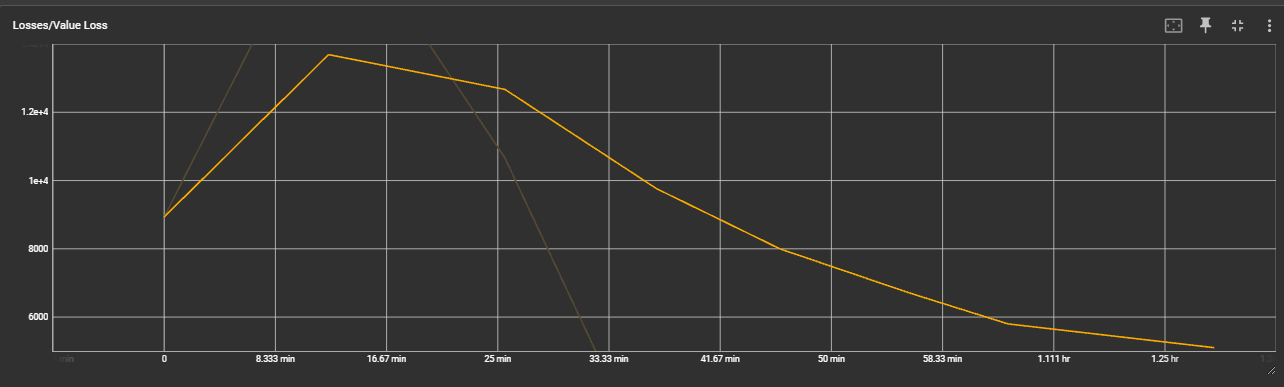
\includegraphics[width=0.8\textwidth]{Figures/NumazuValueLoss.png}
  \caption{価値関数の平均損失} 
  \label{fig:fig-01}
\end{figure}

\end{document}